\documentclass[12pt,a4paper]{article}

% ----------------------------
% Packages
% ----------------------------
\usepackage[margin=1in]{geometry}
\usepackage{setspace}
\usepackage{graphicx}
\usepackage[hidelinks]{hyperref}
\usepackage{titlesec}
\usepackage{fancyhdr}
\usepackage{datetime2}
\usepackage{float}
\usepackage{adjustbox}
\usepackage{rotating}
\usepackage{acronym}
\usepackage{subcaption}
\usepackage{amsmath}
\usepackage{apacite}

% ----------------------------
% Formatting
% ----------------------------
\setstretch{1.2}
\setlength{\parskip}{0.6em}
\setlength{\parindent}{0pt}

\titleformat{\section}
    {\normalfont\Large\bfseries}
    {\thesection}{1em}{}

\titleformat{\subsection}
    {\normalfont\large\bfseries}
    {\thesubsection}{1em}{}

% ----------------------------
% Header / Footer
% ----------------------------
\setlength{\headheight}{15pt}  
\pagestyle{fancy}
\fancyhf{}
\fancyhead[L]{\textit{Quantum Imaging with Undetected Photons}}
\fancyhead[R]{\leftmark}
\fancyfoot[C]{\thepage}

% ----------------------------
% Document Metadata
% ----------------------------
\title{Quantum Imaging with Undetected Photons: Enhanced Image Processing \& User Interface}
\author{Samer Saftawi}
\date{February 2026}

% ----------------------------
% Document
% ----------------------------
\begin{document}

\begin{titlepage}
\centering

\vspace*{2cm}

{\Large\bfseries Thesis Report -- Graduation Internship\par}
\vspace{1.2cm}

{\Huge\bfseries Quantum Imaging with Undetected Photons: Enhanced Image processing \& User Interface\par}

\vspace{4cm}

{\large
\begin{tabular}{@{}l l@{}}
\textbf{Author:} & Samer Saftawi \\
\textbf{Study program:} & Bachelor Applied Computer Science \\
\textbf{Student number:} & 541642 \\
\end{tabular}
}

\vspace{1.5cm}

{\large
\begin{tabular}{@{}l l@{}}
\textbf{Supervisor:} & Dr. D. Polishchuk \\
\textbf{Study Coach:} & Dr. A. Khan \\
\textbf{Research group:} & Applied Nanotechnology \\
\textbf{Project:} & Quantum Delta NL \\
\textbf{Institution:} & Saxion University of Applied Sciences \\
\end{tabular}
}

\vfill

{\large
Internship period: 02.02.2026 -- 03.07.2026\\
}

\end{titlepage}

\newpage

\section*{Abstract}
This graduation internship report, written as part of the Bachelor of Applied Computer Science program at Saxion University of Applied Sciences, presents the development of an enhanced software interface and processing application for a \ac{QIUP} demonstrator. Quantum Photonics is an emerging field that explores the quantum properties of light. \ac{QIUP} is an advanced technique within this field that allows objects to be imaged without directly detecting the photons that interact with them, utilizing quantum entanglement and interference effects. 

In collaboration with the \ac{ANT} research group at Saxion, this project focused on solving the operational bottlenecks of the existing \ac{QIUP} setup. By integrating hardware control and implementing an optimized \ac{FFT} algorithm in Python, the system successfully achieved automated, real-time extraction of phase, visibility and contrast images. The resulting unified graphical user interface significantly reduces setup and acquisition time, giving researchers immediate access to quantitative interference data. Ultimately, this project improves image quality and makes complex quantum imaging technology more accessible for practical demonstrations and research.

\newpage
\section*{Summary}
The aim of this project was to make quantum technologies more accessible to a wider audience by improving a practical quantum imaging demonstrator. Specifically, the project addressed the software limitations of the current \ac{QIUP} setup at Saxion. 

To improve the quality and analytical value of the images produced by the \ac{QIUP} system, an advanced \ac{FFT}-based image processing method, pixel-wise \ac{FFT}, was successfully implemented. Additionally, a cohesive, user-friendly interface was developed to replace the previous manual workflow. This unified application allows users to easily control the camera and the piezoelectric stage, automate data acquisition and visualize the processed visibility, contrast and phase results in real time. 

The final integrated system demonstrated reliable phase extraction, proving that complex quantum optical setups can be operated seamlessly through intuitive software. By streamlining the user experience and automating data analysis, this project enables the broader adoption and demonstration of this cutting-edge technology.

\newpage
\tableofcontents

\newpage

\section*{Abbreviations}
\markboth{LIST OF ABBREVIATIONS}{List of Abbreviations} 
\begin{acronym}[KPZ101] % using the longest acronym for formatting width
    \acro{QIUP}{Quantum Imaging with Undetected Photons}
    \acro{ANT}{Applied Nanotechnology}
    \acro{FFT}{Fast Fourier Transform}
    \acro{TLC}{Talent \& Learning Center}
    \acro{PPLN}{Periodically Poled Lithium Niobate}
    \acro{CMOS}{Complementary Metal-Oxide-Semiconductor}
    \acro{SPDC}{Spontaneous Parametric Down-Conversion}
%    \acro{CCD}{Charged Coupled Device}
    \acro{GUI}{Graphical User Interface}
    \acro{KPZ101}{KCube Piezo Controller}
    \acro{KSG101}{KCube Strain Gauge Meter}
    \acro{SDK}{Software Development Kit}
    \acro{TSI}{Thorlabs Scientific Imaging}
    \acro{CLR}{Common Language Runtime}
    \acro{SNR}{Signal-to-Noise Ratio}
    \acro{FFTW}{Fastest Fourier Transform in the West}
    \acro{SIMD}{Single Instruction, Multiple Data}
    \acro{ROI}{Region Of Interest}
\end{acronym}

\newpage
\section*{List of Figures and Tables}
\listoffigures
\listoftables

\newpage
\section{Introduction}
This chapter provides an introduction to the project, explains the background and context of the assignment and describes the setup of the demonstrational platform for \ac{QIUP} at the \ac{TLC} lab within the \ac{ANT} research group.

\subsection{Background of the Assignment}
    As part of the QDNL program, this project aims to accelerate the development and adoption of quantum technologies \cite{quantum_delta}.
    A primary challenge in this field is the non-intuitive nature of quantum properties such as entanglement and indistinguishability. These properties are leveraged in \ac{QIUP} to enable imaging without directly interacting with the photon that detects the sample.

    The demonstrational setup for \ac{QIUP} at the \ac{TLC} lab within the \ac{ANT} research group provides a platform for exploring and enhancing this technology.

\subsection{The Setup}
    The experimental implementation of the quantum imager is shown in Figure \ref{fig:demonstrator}. 
    The system consists of:

    \begin{itemize}
    \item Continuous-wave pump laser
    \item \ac{PPLN} nonlinear crystal
    \item Dichroic beam splitter
    \item Piezoelectric-stage connected to a mirror
    \item Thorlabs Zelux \ac{CMOS} camera
    \end{itemize}

    \begin{figure}[H]
    \centering
    \begin{subfigure}[b]{1\linewidth}
        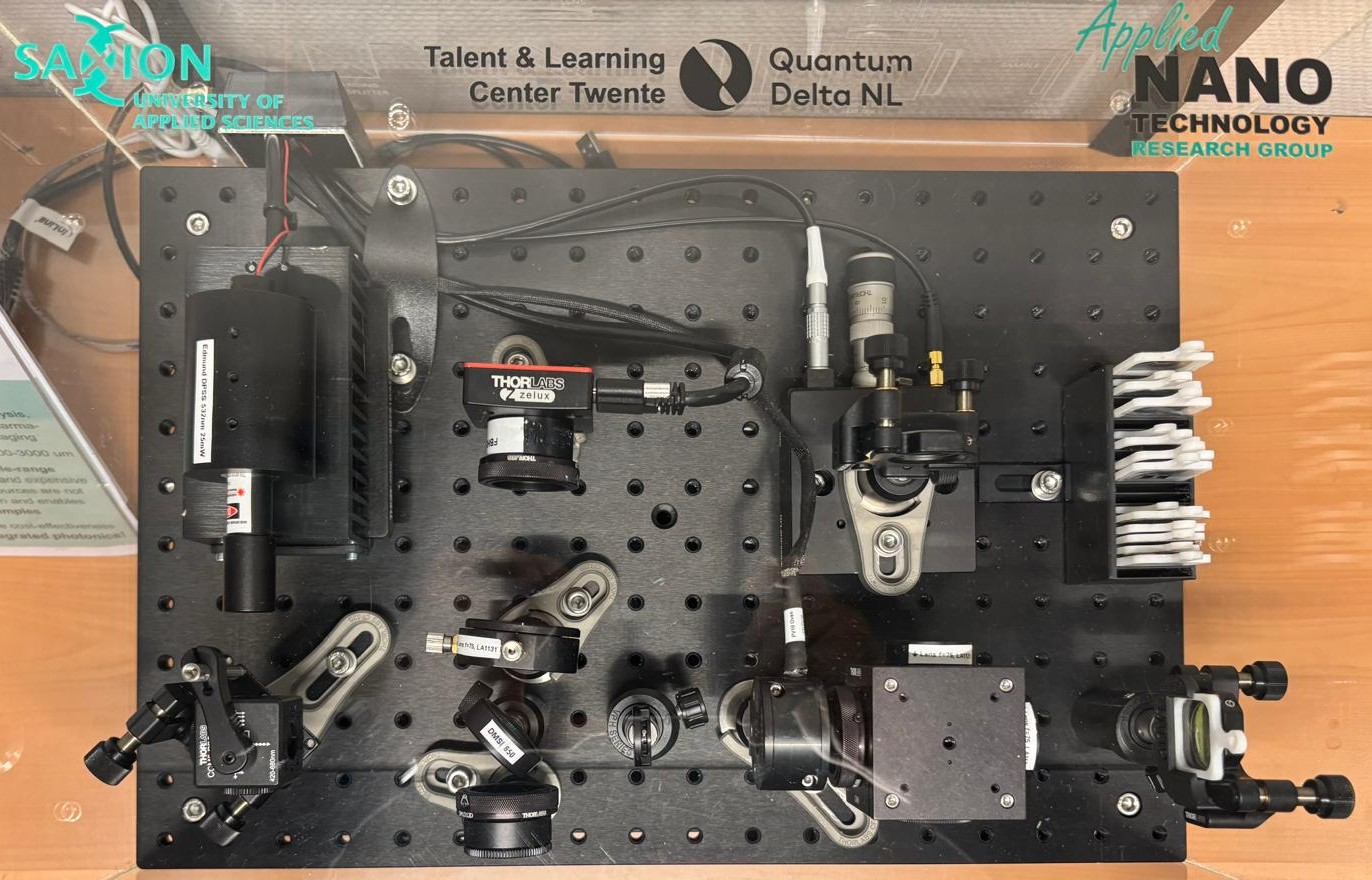
\includegraphics[width=\linewidth]{images/setup/demonstrator_setup.jpeg}
        \caption{Top-Down view on demonstrational setup at Saxion.}
    \end{subfigure}
    \begin{subfigure}[b]{1\linewidth}
        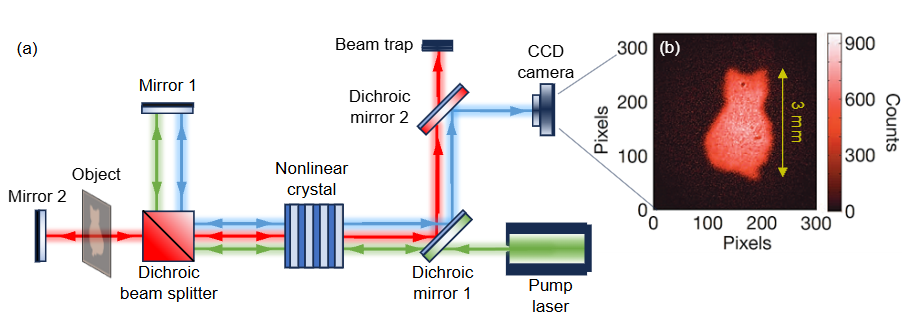
\includegraphics[width=\linewidth]{images/setup/setup_schematic.png}
        \caption{Schematic of demonstrational setups functionality.}
    \end{subfigure}
    \caption{Demonstrational Setup and Schematic.}
    \label{fig:demonstrator}
    \end{figure}

    The system relies on the principle of induced coherence, utilizing a nonlinear interferometer.

    As detailed in the schematic (Figure \ref{fig:demonstrator}b), a continuous wave pump laser is directed into a nonlinear crystal (specifically, a \ac{PPLN} crystal). Through \ac{SPDC}, the pump photon splits into a signal photon (visible spectrum) and an idler photon (infrared). A dichroic beam splitter separates these paths: the visible signal is reflected by a reference mirror (Mirror 1), while the infrared idler interacts with the target object before being reflected by Mirror 2.
    
    The idler photons that pass through the object contain spatial information about its absorption or phase profile. When the idler and signal beams recombine at the crystal, quantum interference modulates the intensity of the signal beam based on the idler's path information. Consequently, the image of the object, which was only "seen" by the infrared light, is transferred to the visible spectrum and detected by the camera.
    
    The physical realization of this schematic is shown in Figure \ref{fig:demonstrator}a. The setup is constructed on an optical breadboard to ensure stability. The pump source directs the beam through conditioning optics towards the central crystal mount. The detection module utilizes a Thorlabs Zelux \ac{CMOS} camera to capture the interference patterns. 


\subsection{Problem Definition and Objectives}

    In this section, the specific challenges and goals of the project are defined. The current \ac{QIUP} setup, while functional, has limitations in terms of image quality and user accessibility.
    \subsubsection{Problem Definition}
    The experimental setup for \ac{QIUP} serves as a powerful proof-of-concept for mid-infrared imaging. 
    However, the current setup has practical limitations regarding image quality and user accessibility.
    Currently, two main software tools provided by Thorlabs are used to control the setup and process the images: Thorcam \cite{ThorlabsThorCam} (left part of Figure \ref{fig:old_showcase}) and Kinesis \cite{ThorlabsKinesis} (right part of Figure \ref{fig:old_showcase}). These are used for separate camera and piezoelectric actuator control, but they are not optimized for \ac{QIUP} applications or advanced image processing.
    
    Using this approach is unintuitive and requires significant manual effort just to obtain grayscale images. Furthermore, the resulting image quality is limited, as illustrated in Figure \ref{fig:old_showcase}.

    \begin{figure}[H]
    \centering
        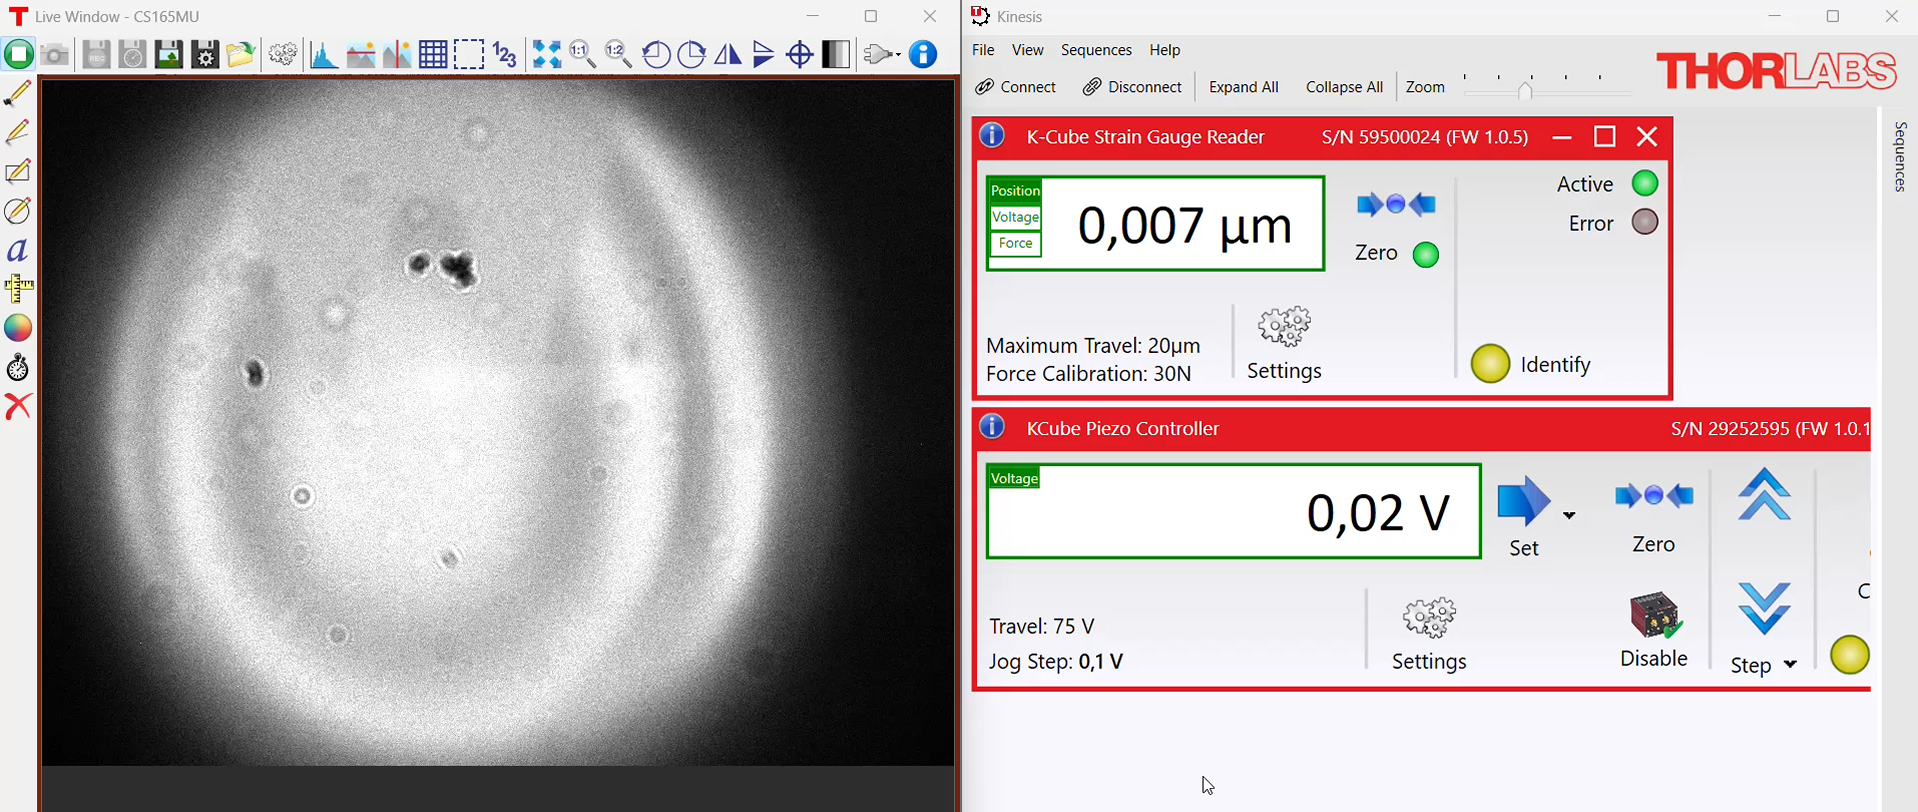
\includegraphics[width=0.8\linewidth]{images/old_showcase.png}
        \caption{Old Showcase of the QIUP Setup.}
        \label{fig:old_showcase}
    \end{figure}

    \subsubsection{Objectives}
    The main objective of this project is to transform the current laboratory setup into a robust, automated and user-friendly demonstrator platform. This goal is divided into the following sub-objectives:
        \begin{enumerate}
            \item \textbf{Advanced Image Processing:} Process captured images using mathematical techniques, specifically the \ac{FFT}, to enhance image quality and extract detailed information like visibility, contrast and phase from the raw data.
            \item \textbf{Hardware Automation System:} Streamline the current use of multiple software tools into a single, cohesive Python application that manages camera control, piezoelectric actuators and data acquisition.
            \item \textbf{User Interface Development:} Develop a user-friendly interface to allow researchers and students to easily interact with the \ac{QIUP} system. The interface will provide intuitive controls for operating the hardware and visualizing key metrics in real time.
        \end{enumerate}

\subsection{Scope of Work}
    To determine the success of this project, the expected technical results have been categorized using the MoSCoW method:

    \textbf{Must Have:}
    \begin{itemize}
        \item Hardware Automation System: A Python-based control script capable of communicating with and reliably driving both the Thorlabs \ac{CMOS} camera and the piezoelectric stage.
        \item Image Processing Core: A functional \ac{FFT}-algorithm capable of reconstructing visibility, contrast and phase images from raw sensor data.
    \end{itemize}

    \textbf{Should Have:}
    \begin{itemize}
        \item Functional \ac{GUI}: An intuitive interface that allows the operator to control the hardware, acquire live images and display the processed quantum interference patterns.
        \item Performance Optimization: Optimized code execution that ensures image processing is fast enough for smooth, live audience demonstrations.
        \item Advanced Camera Settings: The ability to adjust camera settings (exposure time, gain, frame rate) directly through the custom software interface.
    \end{itemize}

    \textbf{Could Have:}
    \begin{itemize}
        \item Advanced \ac{GUI} Capabilities: Additional features such as calibration presets, advanced data visualization tweaks, or data export functions.
        \item New Samples: The introduction of new samples (transparent or opaque) to better showcase the capabilities of the \ac{QIUP} technology during demonstrations. 
    \end{itemize}

    \textbf{Won't Have:}
    \begin{itemize}
        \item Hardware Upgrades: The physical integration of new hardware components not present in the current optical setup.
    \end{itemize}

\subsection{Approach \& Methodology}

    This project combines software development with experimental physics validation. To manage the iterative nature of development alongside hardware integration, the project utilizes the Scrum framework. This allows for flexibility while ensuring continuous delivery of features and frequent testing on the physical setup.

    \subsubsection{Development Process}
    The project is divided into sprints lasting 1--4 weeks. This duration provides a balance between sufficient development time and frequent feedback loops. At the end of each sprint, the results are reviewed and the subsequent sprint is adjusted based on integration progress.

    \subsubsection{System Architecture and Tools}
    The software is developed as a modular system using the following tools:
    \begin{itemize}
        \item \textbf{Language \& IDE:} Python is used for the entire system development within the Visual Studio Code environment.
        \item \textbf{Hardware Control:} Integration with the Thorlabs piezoelectric stage (KPZ101/KSG101) and \ac{CMOS} camera is handled via the Kinesis .NET API and ThorCam SDK.
        \item \textbf{Data Management:} Project assets are saved in a secure directory on the \ac{ANT} internal network, ensuring data integrity and unified access.
    \end{itemize}

    \subsection{Outline of the Report}
    \begin{enumerate}
        \item \textbf{Introduction:} Provides background on quantum imaging technology, defines the problem statement, outlines project objectives and presents the methodology and scope of work.
        \item \textbf{Analysis / Specifications:} Details the requirements analysis, system specifications and constraints for the enhanced image processing and user interface development.
        \item \textbf{Functional Design:} Describes the functional architecture, user workflows and feature specifications for the image processing algorithms and UI components.
        \item \textbf{Technical Design:} Presents the technical implementation approach, software architecture, technology stack and design patterns used for the project.
        \item \textbf{Realisation:} Documents the actual implementation of the system, including code development, integration and deployment of the software.
        \item \textbf{Testing:} Covers testing strategies, test cases, results and validation of the image processing quality and user interface functionality.
        \item \textbf{Conclusions \& Recommendations:} Summarizes key findings, evaluates achievement of objectives and provides recommendations for future improvements.
    \end{enumerate}

\newpage

\section{Analysis and Specifications}
    In this chapter, the system requirements and constraints for the \ac{QIUP} demonstrator project are analyzed. To contextualize these technical specifications, it is important to first understand the underlying physical principles that enable \ac{QIUP} technology.
        
    \subsection{Physical Specifications}
    There are many complex quantum phenomena at play in the \ac{QIUP} system, but the following key principles are essential to understand the image formation process and the resulting data that the software will analyze.
        
    \subsubsection{Nonlinear Interferometry} 
        The foundation of \ac{QIUP} relies on the nonlinear interferometer. 
        While a standard classical interferometer utilizes conventional beam splitters to divide and recombine light to measure interference patterns, a nonlinear interferometer replaces these with nonlinear crystals. This allows the system to exploit the quantum properties of light, specifically generating and correlating photon pairs \cite{NonlinearInterferometry}.
        
    \subsubsection{Spontaneous Parametric Down-Conversion (SPDC)}
        The core physical mechanism driving this system is \ac{SPDC} \cite{lemos2014quantum}. 
        When a pump laser illuminates a specialized nonlinear crystal (in this setup, a \ac{PPLN} crystal), pump photons spontaneously split into pairs of lower-energy photons \cite{NonlinearInterferometry}. These newly created photons are designated as the signal and the idler. For this demonstrator, the signal photon lies within the visible spectrum and is detected by a standard \ac{CMOS} camera, whereas the idler photon is generated in the infrared spectrum and probes the sample.
        
    \subsubsection{Induced Coherence and ``Which-Way'' Information}
        The theoretical framework of \ac{QIUP} is built upon the phenomenon of ``induced coherence without induced emission'' \cite{lemos2014quantum, NonlinearInterferometry}. The optical setup is configured such that a signal-idler photon pair can be probabilistically generated either in the first pass through the crystal or the second (after reflection). The system is precisely aligned so that the emission path of the idler from the first potential origin overlaps perfectly with the emission path from the second. 
        
    \subsubsection{Indistinguishability and Interference}
        Quantum interference patterns manifest on the camera only if the origin of the detected photon remains fundamentally unknown \cite{NonlinearInterferometry, lemos2014quantum}. By overlapping the infrared idler beams, the setup intentionally erases the ``which-way'' (welcher-weg) information regarding the photon pair's origin \cite{lemos2014quantum}. This spatial indistinguishability induces coherence between the visible signal photons, enabling them to interfere despite never having interacted with the sample \cite{pearce2023practical, NonlinearInterferometry}. 
    
    \subsubsection{Extracting the Image}
        To utilize this quantum phenomenon for imaging, a sample is placed solely in the path of the infrared idler photon. The idler photon gathers the physical information about the object but is entirely discarded without reaching a detector \cite{lemos2014quantum}. Meanwhile, the visible signal photon never interacts with the object, yet its interference pattern, captured by the \ac{CMOS} camera and processed via \ac{FFT}, contains the complete spatial information of the sample \cite{kutas2021quantum, pearce2023practical}.
                    
    \subsubsection{Spectral Leakage} 
        Spectral leakage is an analytical artifact that occurs during the \ac{FFT} processing of the phase-shifted image stack. 
        It arises when the piezoelectric phase scan does not capture an exact integer number of interference cycles. Because the \ac{FFT} algorithm assumes the finite sampled signal is periodically infinite, a mismatch causes the signal's energy to spread or "leak" into adjacent Fourier components. This leads to an underestimation of the primary interference amplitude, artificially degrading the calculated visibility, contrast and phase. Hence, accurate calibration of the phase scan is required to maximize image quality \cite{SpectralLeakageEssentials}.

    \subsubsection{Visibility, Contrast and Phase Reconstruction} 
        By applying Fourier-transform techniques to the captured phase-shifted image stack, three distinct quantitative images can be reconstructed. In practice, this involves analyzing the intensity variations pixel-by-pixel as the interference patterns change. For a given pixel, let $N_{max}$ and $N_{min}$ represent the maximum and minimum recorded intensity values, while $F_1$ and $F_0$ represent the amplitude of the primary interference frequency and the DC component derived from the \ac{FFT} \cite{pearce2023practical}. The parameters are calculated as follows:
        
        \begin{itemize}
            \item \textbf{Visibility Image:} Fringe visibility shows the strength of the quantum interference. In \ac{QIUP}, visibility is fundamentally linked to the opacity of the sample. If the sample absorbs or scatters the infrared idler photon, the ``which-way'' information becomes distinguishable, causing a localized drop in interference visibility \cite{lemos2014quantum, NonlinearInterferometry}. Visibility $V$ is calculated as:
            \begin{equation}
                V = \frac{N_{max}-N_{min}}{N_{max}+N_{min}} = \frac{N_{amp}}{N_{mean}} = \frac{2F_{1}}{F_{0}}
                \label{eq:visibility}
            \end{equation}
            where $N_{amp}$ is the amplitude of the interference oscillation and $N_{mean}$ is the average pixel intensity \cite{pearce2023practical}.
            
            \item \textbf{Contrast Image:} Closely related to visibility, contrast provides an alternative metric that is particularly useful in systems with a higher noise floor, as the mean background intensity is subtracted rather than used as a denominator. The contrast $C$ is mathematically defined as:
            \begin{equation}
                C = N_{max}-N_{min} = 2N_{amp} = 4F_{1}
                \label{eq:contrast}
            \end{equation}
            This amplitude map provides a robust representation of the sample's transmission characteristics \cite{pearce2023practical, xie2018surface}.
            
            \item \textbf{Phase Image:} The phase of the interference pattern shifts in direct response to changes in the optical path length experienced by the idler photon as it traverses the sample. The phase shift $\phi$ is extracted using the real (Re) and imaginary (Im) parts of the fundamental Fourier component $F_1$:
            \begin{equation}
                \phi = \arctan\left(\frac{\text{Im}(F_{1})}{\text{Re}(F_{1})}\right)
                \label{eq:phase}
            \end{equation}
            This enables quantitative phase imaging of an object in the infrared regime using only visible light detection \cite{pearce2023practical}.
        \end{itemize}

    \subsection{Hardware Specifications}
    The demonstrational setup integrates several hardware components essential for the operation of the \ac{QIUP} system. This section details the specifications of the programmable hardware interfaces: the piezoelectric translation stage and the \ac{CMOS} camera.

        \subsubsection{Piezoelectric Stage}
        To utilize the principle of induced coherence, the setup relies on a piezoelectric stage to precisely modulate the optical path length of the signal beam. Because the detected signal wavelength is roughly 810 nm, creating stable phase shifts requires nanometer adjustments.
        
        \begin{itemize}
            \item \textbf{Thorlabs \ac{KPZ101} Piezoelectric Controller:}
                \begin{figure}[H]
                    \centering
                    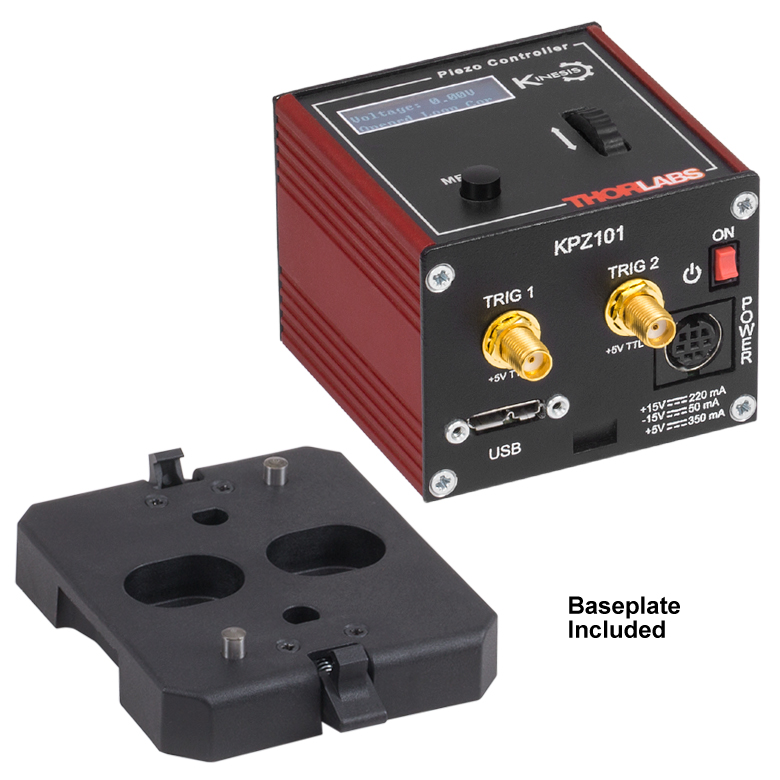
\includegraphics[width=0.45\linewidth]{images/components/KPZ101.jpg}
                    \caption{Thorlabs \ac{KPZ101} Piezoelectric Controller.}
                    \label{fig:KPZ101}
                \end{figure}
                The \ac{KPZ101} controls the displacement of the piezoelectric actuator by applying precise voltages. This enables the smooth expansion or contraction of the stage, shifting the optical path length of the signal beam to generate the necessary interference sweep \cite{ThorlabsKPZ101}. The \ac{KPZ101} is visualized in Figure \ref{fig:KPZ101}.

            \item \textbf{Thorlabs \ac{KSG101} Strain Gauge Meter:}
                \begin{figure}[H]
                    \centering
                    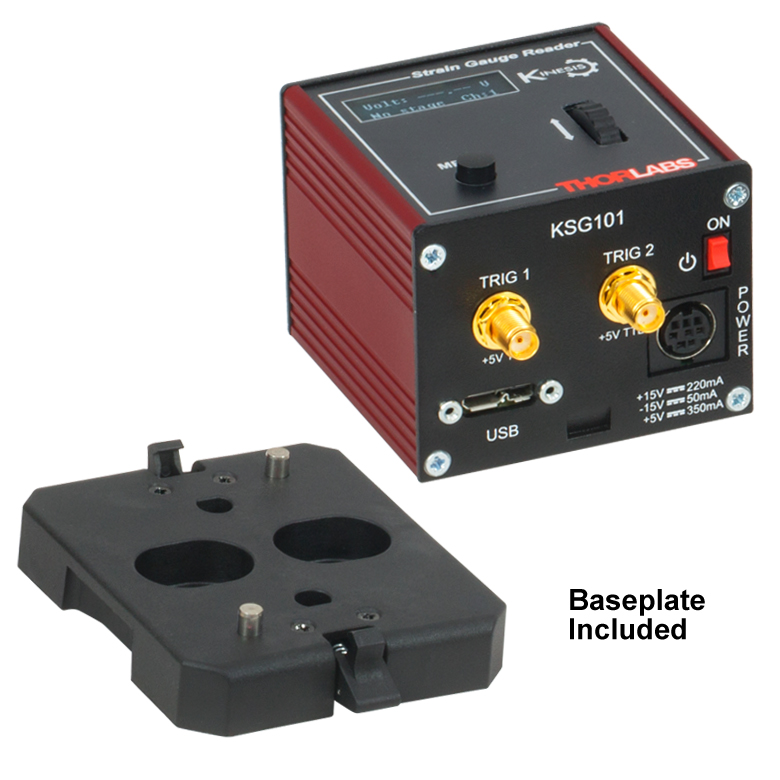
\includegraphics[width=0.45\linewidth]{images/components/KSG101.jpg}
                    \caption{Thorlabs \ac{KSG101} Strain Gauge Meter.}
                    \label{fig:KSG101}
                \end{figure}
                Because piezoelectric materials suffer from inherent hysteresis, the \ac{KSG101} provides real-time positional feedback. It measures the physical strain on the actuator, ensuring the exact scanning travel distance is achieved. This feedback helps capture exactly one interference cycle, mitigating spectral leakage during \ac{FFT} analysis \cite{ThorlabsKSG101}. The \ac{KSG101} is visualized in Figure \ref{fig:KSG101}. 
        \end{itemize}

        \subsubsection{CMOS Camera}
        A Thorlabs Zelux \ac{CMOS} camera, operating at a resolution of $1440 \times 1080$ pixels, serves as the primary detector to record the spatial distribution of the visible signal photons. The sensor captures the interference modulations across its pixel array, providing the raw matrix data necessary for the pixel-wise \ac{FFT} transformations.
        
        \begin{figure}[H]
            \centering
            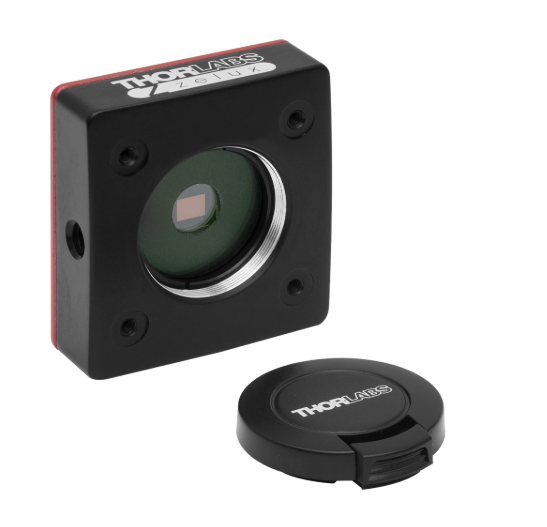
\includegraphics[width=0.45\linewidth]{images/components/CMOS.png}
            \caption{Thorlabs Zelux CMOS Camera.}
            \label{fig:CMOS}
        \end{figure}
    
    \subsection{Software Specifications}
        To control the hardware components and process the acquired image stacks efficiently, a specific software architecture is required. Python was selected as the foundational language because it natively supports a wide range of optimized scientific libraries and is highly accessible for future researchers.

        \subsubsection{Software Development Kits} 
            To integrate hardware control seamlessly into Python, two primary \ac{SDK}s from Thorlabs are utilized. 
            First, the \ac{TSI} Camera Python \ac{SDK} serves as the interface for the Zelux \ac{CMOS} camera, granting direct programmatic access to critical parameters like exposure time and gain. Importantly, the \ac{TSI} \ac{SDK} allows the direct acquisition of sensor data into Python memory as multidimensional NumPy arrays \cite{TSIDocs}. 
            
            Second, precision motion control relies on the Thorlabs Kinesis .NET API. Using the \texttt{pythonnet} bridge module, the application loads the \ac{CLR} directly into the Python backend. This allows the software to issue closed-loop positional commands to the \ac{KPZ101} while simultaneously monitoring the \ac{KSG101} feedback \cite{KinesisInPython}.
        
        \subsubsection{FFT-Based Image Processing}
            In a \ac{QIUP} demonstrator, the most important information is found in how the image changes over time. Because the system utilizes an interferometer with a scanning piezoelectric stage, the light intensity at any given point oscillates sinusoidally as the optical path length changes, creating moving interference fringes \cite{xie2018surface}.

            To translate these interferometric effects into clear visibility, contrast and phase maps, this project implements a pixel-wise \ac{FFT} approach. Rather than analyzing the spatial patterns of a single frame, every individual coordinate on the detection plane is treated as an independent sensor, tracking how the brightness changes over a sequence of frames.
    
    \subsection{Requirements}
    This section specifies the criteria that the final software and hardware combination must satisfy, categorized into User Requirements and System Requirements.

    \subsubsection{User Requirements}
    User requirements define the operational capabilities needed to successfully conduct \ac{QIUP} demonstrations.

    \begin{table}[H]
        \centering
        \renewcommand{\arraystretch}{1.3}
        \begin{tabular}{|p{0.1\linewidth}|p{0.65\linewidth}|p{0.15\linewidth}|}
            \hline
            \textbf{ID} & \textbf{Requirement Description} & \textbf{Priority} \\ \hline
            UR-01 & The user must be able to view live, reconstructed visibility, contrast and phase images within a single \ac{GUI}. & Must \\ \hline
            UR-02 & The user must be able to initiate an automated, synchronized hardware phase-scan sequence. & Must \\ \hline
            UR-03 & The user should be able to adjust camera parameters (e.g., exposure time, gain) directly from the dashboard. & Should \\ \hline
            UR-04 & The user should experience responsive software feedback with low processing delays. & Should \\ \hline
            UR-05 & The user could have the ability to explicitly save or export the processed numerical data and visual images. & Could \\ \hline
        \end{tabular}
        \caption{User Requirements for the QIUP setup.}
        \label{tab:user_requirements}
    \end{table}

    \subsubsection{System Requirements}
    System requirements dictate the technical targets the system architecture must achieve.
    
    \begin{table}[H]
        \centering
        \renewcommand{\arraystretch}{1.3}
        \begin{tabular}{|p{0.1\linewidth}|p{0.65\linewidth}|p{0.15\linewidth}|}
            \hline
            \textbf{ID} & \textbf{Requirement Description} & \textbf{Priority} \\ \hline
            SR-01 & The system must establish a stable connection to the \ac{CMOS} camera using the \ac{TSI} \ac{SDK}, capturing frames into NumPy memory. & Must \\ \hline
            SR-02 & The system must execute motion control via the Kinesis API, utilizing the \ac{KSG101} feedback for target displacements. & Must \\ \hline
            SR-03 & The system must synchronize camera acquisition with piezo stepping to capture exactly one full interference cycle. & Must \\ \hline
            SR-04 & The system must ingest the resulting image stack and execute a pixel-wise \ac{FFT} to isolate the DC and AC components per pixel. & Must \\ \hline
            SR-05 & The system should utilize the PyFFTW library to complete the image stack processing pipeline with minimal latency (e.g., $\le 200$ ms). & Should \\ \hline
        \end{tabular}
        \caption{System Requirements for the QIUP setup.}
        \label{tab:system_requirements}
    \end{table}

\newpage

\section{Functional Design}
To demonstrate how the system fulfills the specified requirements, this chapter outlines the functional design of the software and hardware integration for the \ac{QIUP} demonstrator application. 
This architecture serves as the foundation for the technical design. The overall system functionality is divided into three primary modules: hardware control, image processing and the user interface. 

    \subsection{System Overview}
    A high-level understanding of the interactions between individual system components is essential. The system combines hardware control and data processing within a single \ac{GUI}. This interface manages both the piezoelectric stage controllers and the \ac{CMOS} camera. The piezo stage controls the optical path length of the signal photon, altering the interference pattern, while the camera captures the intensity variations at each position. In addition, the application incorporates advanced image processing to analyze this raw data, calculating visibility, contrast and phase information.

    The software architecture prioritizes usability, enabling operators to control hardware, acquire datasets and visualize processed results. The operational workflow begins with hardware initialization. Following successful initialization, the \ac{GUI} provides control over camera settings (such as exposure time and gain) and defines the travel range for the piezo stage. The interface includes real-time feedback monitoring, presenting intensity variations within a user-defined Region of Interest.

    To ensure optimal experimental conditions, users can access the live camera feed for initial optical alignment. This preview is critical for verifying the presence of interference fringes and confirming that the sample is correctly positioned, which are strict prerequisites for robust processing.

    Upon completing the setup, the user can initiate an automated phase-scanning sequence, selecting either a single-acquisition scan or a live-acquisition scan. This sequence translates the piezo stage through predefined steps, capturing an image stack. This stack is subsequently processed using a pixel-wise \ac{FFT} algorithm to reconstruct spatial visibility, contrast and phase maps, which are rendered in real-time. 
    
    Finally, the software ensures that all hardware components are safely disconnected when the program is closed and provides options to save acquired data for future analysis (Figure \ref{fig:high_level_overview}).

    \begin{figure}[H]
        \centering
        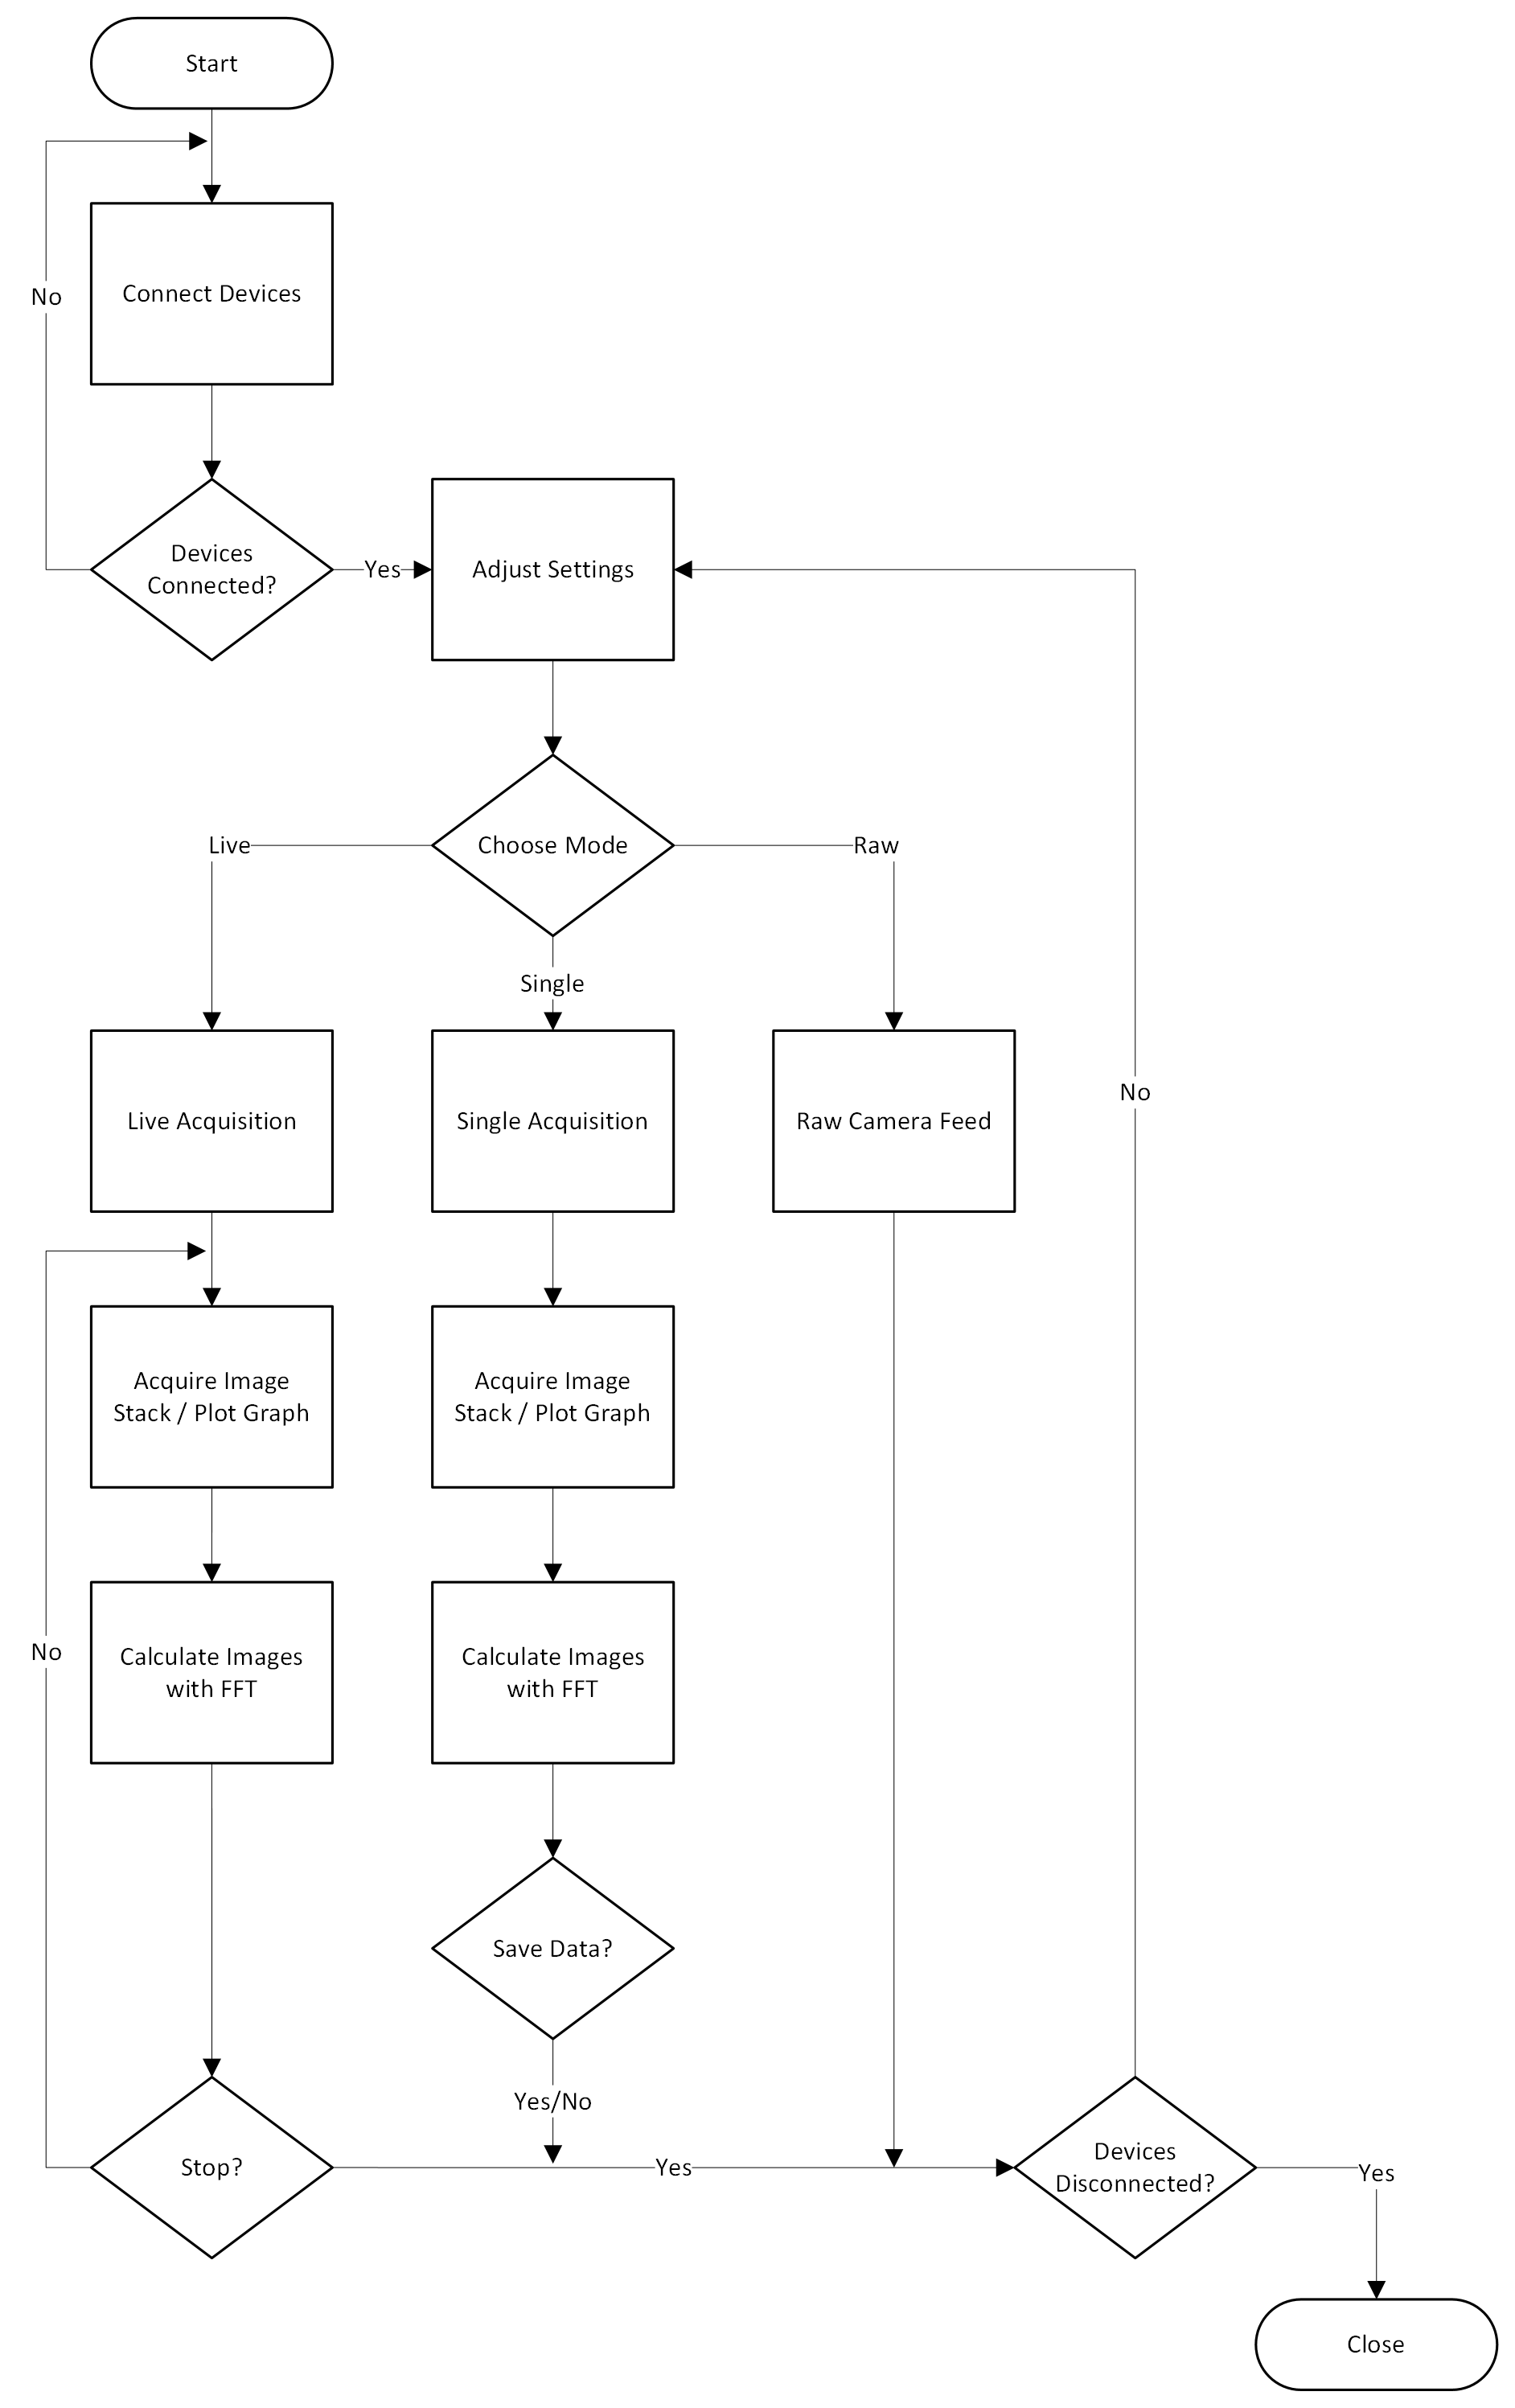
\includegraphics[width=0.9\linewidth]{images/graphs/QIUP System Overview.png}
        \caption{High-level overview of the \ac{QIUP} system architecture and operational workflow.}
        \label{fig:high_level_overview}
    \end{figure}

\subsection{Piezoelectric Stage Control}
    The functional objective of the piezoelectric stage is to execute precise and repeatable phase scanning. This mechanical movement is critical for leveraging induced coherence, ensuring the acquired image stack contains the interferometric modulation required for \ac{FFT} processing. To accommodate different experimental needs, the system supports two operational modes: open-loop and closed-loop control. 
    
    The operational workflow (Figure \ref{fig:piezo_functionality}) begins with the user defining scan parameters (travel distance and number of frames). The system calculates the required voltage steps or target displacements, enters an automated loop to move the stage, verifies the position (if in closed-loop mode) and triggers the camera. Upon completion, the stage automatically resets.

    \begin{figure}[H]
        \centering
        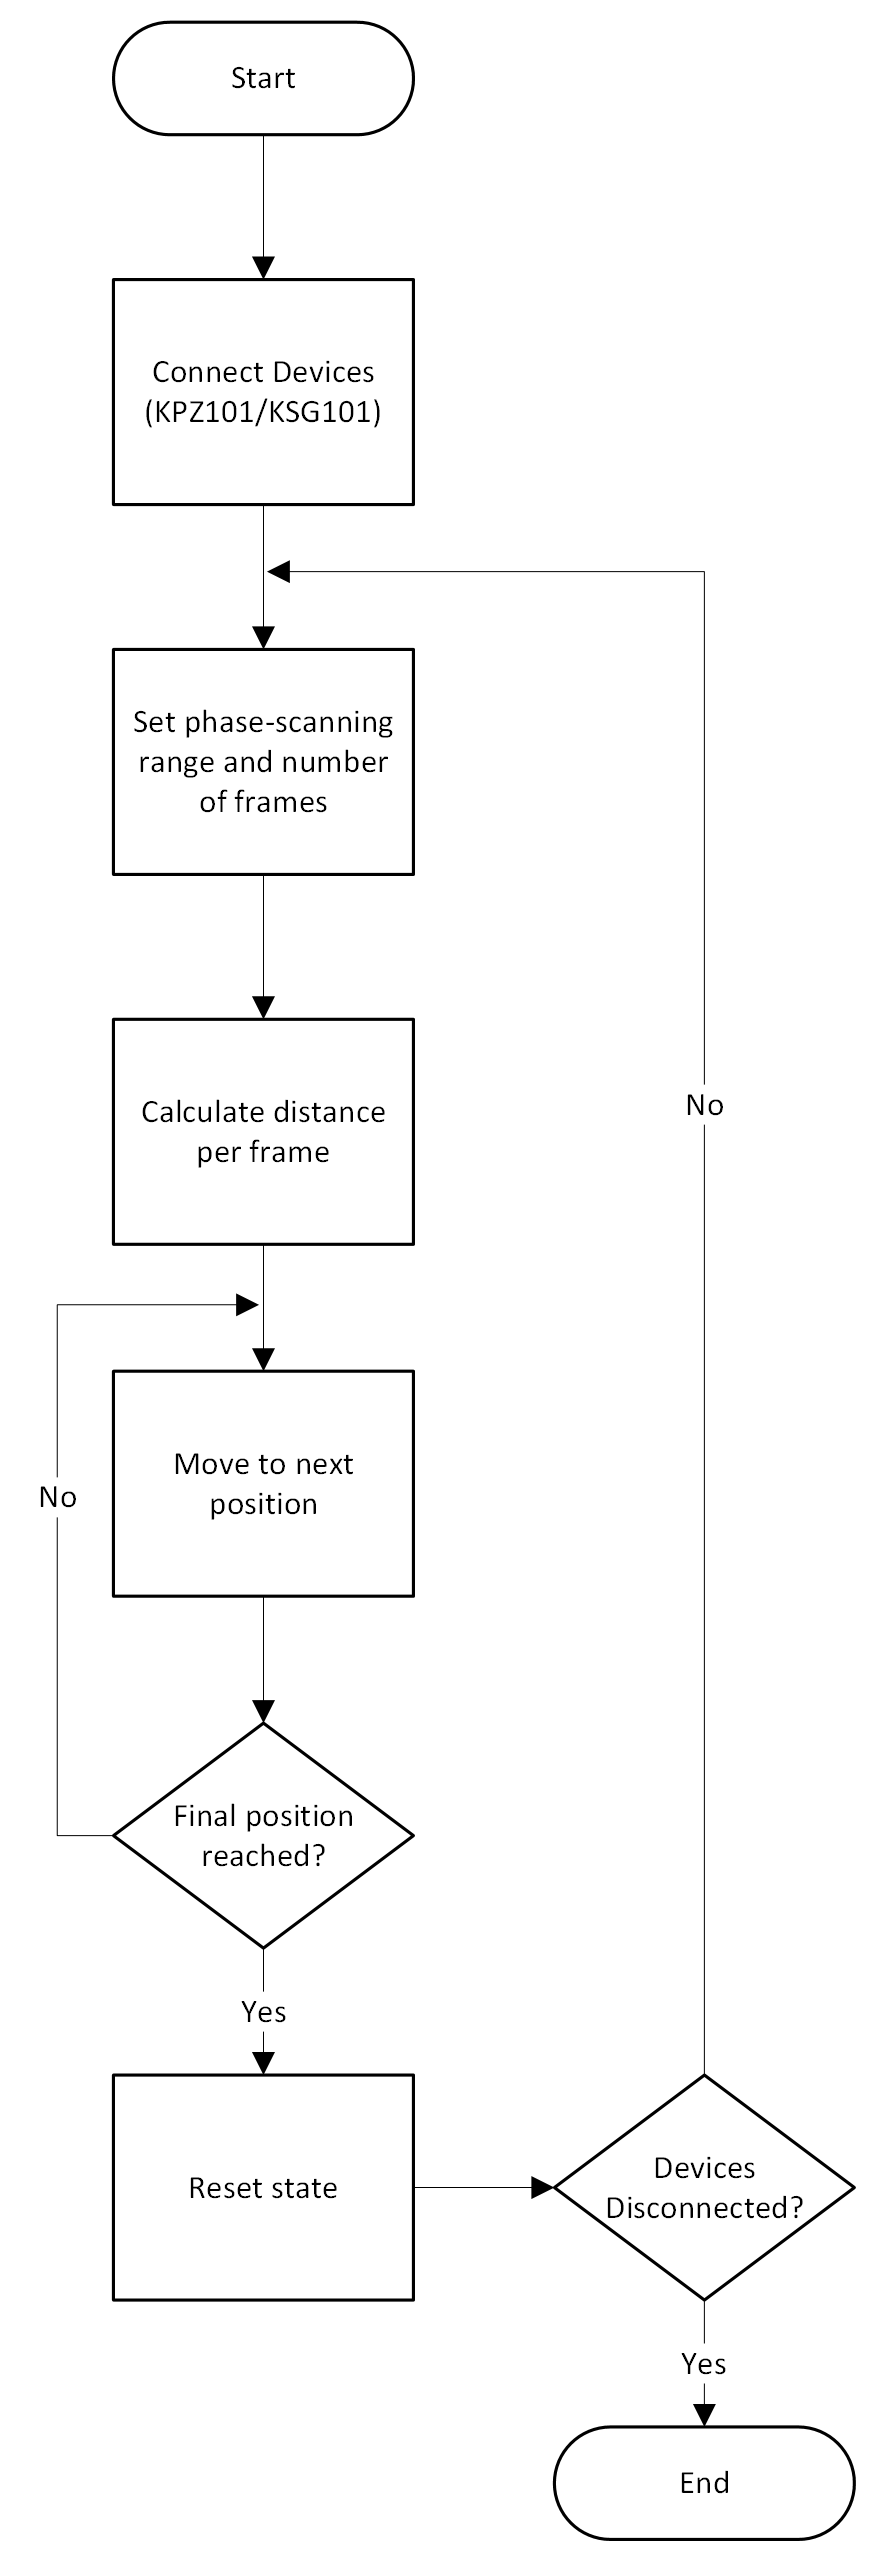
\includegraphics[width=0.45\linewidth]{images/graphs/Piezo Functionality.png}
        \caption{Functional diagram detailing the operational workflow for the piezoelectric stage.}
        \label{fig:piezo_functionality}
    \end{figure}
    
\subsection{Acquisition Methods}
    The fundamental functional requirement of the \ac{QIUP} demonstrator is the reliable acquisition of phase-shifted image sequences. To facilitate near real-time image reconstruction, the acquisition block must continuously capture raw sensor data directly into the system's memory with minimal latency. 

    Prior to initiating a scan, the camera's acquisition parameters must be configured. In a \ac{QIUP} setup, the visible signal generated via \ac{SPDC} inherently exhibits a low photon flux. Therefore, careful adjustment of the camera's exposure time and gain is necessary to maximize the \ac{SNR}:

    \begin{itemize}
        \item \textbf{Exposure Time:} The exposure time balances signal accumulation against environmental noise. It should be long enough to collect sufficient photons, but short enough to avoid pixel saturation (which distorts \ac{FFT} analysis) and to minimize motion blur caused by thermal drift.
        \item \textbf{Gain:} Appropriate analog gain levels boost the faint interferometric fringes above the digital noise floor. However, excessive gain disproportionately inflates background noise and degrades the computed contrast.
    \end{itemize}   

    Functionally, the architecture allows the operator to dynamically adjust these parameters while observing a live video feed. Once the optimal \ac{SNR} is confirmed, the system supports two distinct acquisition modes:
    
    \begin{itemize}
        \item \textbf{Single Acquisition Mode:} The piezo stage moves through predefined steps, capturing a discrete stack of images. This is ideal for detailed examination of specific samples where maximum image quality is desired.
        \item \textbf{Live Acquisition Mode:} The system transitions into a continuous loop to capture and process a real-time sequence of images until manually stopped. This is particularly useful for live demonstrations.
    \end{itemize}

    The general acquisition workflow is illustrated in Figure \ref{fig:acquisition_functionality}. 

    \begin{figure}[H]
        \centering
        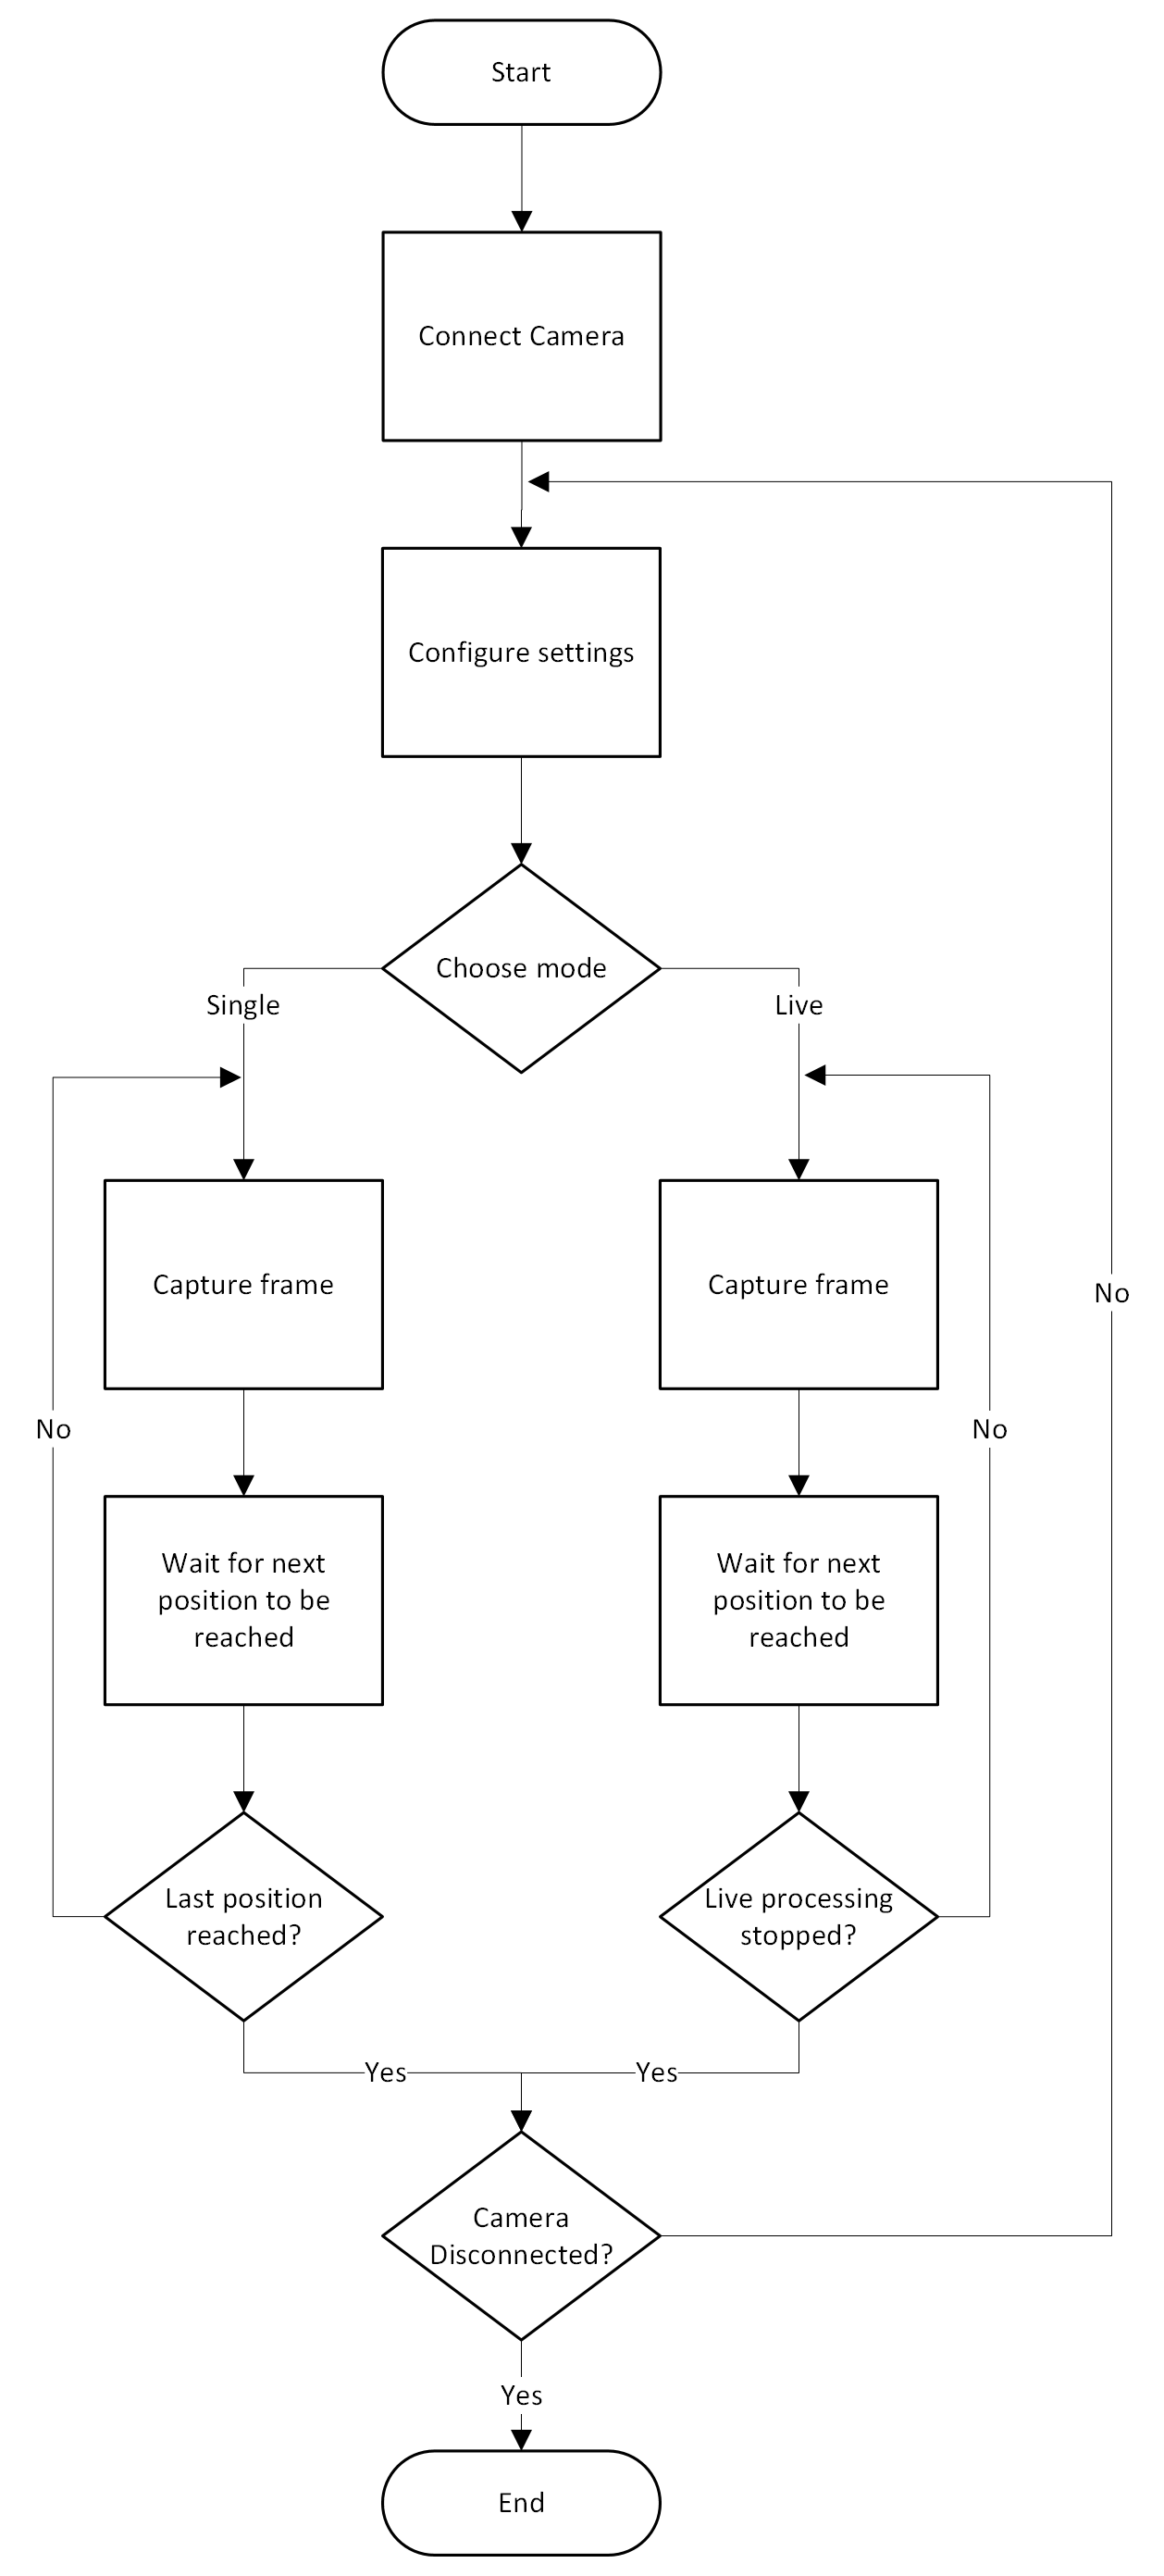
\includegraphics[width=0.65\linewidth]{images/graphs/Acquisitions functionality.png}
        \caption{Functional diagram detailing the operational workflow for the acquisition methods.}
        \label{fig:acquisition_functionality}
    \end{figure}

    \subsection{Image Processing: Pixel-Wise Temporal FFT}
    To extract quantitative metrics from a phase-shifted image sequence, the image processing relies on a pixel-wise temporal \ac{FFT}.
    
    Rather than analyzing an entire interferogram as a single 2D spatial entity, this approach treats every individual coordinate on the detection plane as an independent temporal signal. As the optical path length sweeps through a phase cycle, the intensity at coordinate $(x,y)$ oscillates, creating a discrete 1D temporal wave. Applying a 1D \ac{FFT} along this phase axis isolates the fundamental components per pixel: the static background intensity ($F_0$), the amplitude of the interference oscillation ($F_1$) and the relative phase shift ($\phi$). The final spatial maps are reconstructed by aggregating these independently processed points.
    
    \textbf{Advantages of 1D Temporal FFT over 2D Spatial FFT} \\
    A 2D spatial \ac{FFT} analyzes geometric frequencies (e.g., edges, textures and spatial gradients of an object). If the target sample possesses a complex spatial structure, its inherent geometric frequencies can overlap with the spatial frequency of the quantum fringes, making accurate signal separation prone to errors.
    
    By using a 1D temporal (pixel-wise) \ac{FFT}, the spatial complexity of the object is completely decoupled from the interference signal. The quantum information is strictly encoded in the temporal phase-shift induced by the scanning interferometer, independent of the spatial geometry of the frame.
    
    The main advantage of isolating dynamic temporal frequencies on a per-pixel basis extends well beyond quantum photonics. For instance, recent architectures in computer vision utilize pixel-wise temporal Fourier transforms to detect deepfake videos \cite{kim2025beyond}. Just as \ac{QIUP} utilizes this method to isolate quantum interference, these detection frameworks apply 1D temporal \ac{FFT}s to uncover fluctuations in the pixel plane that traditional 2D spatial frequency analysis does not capture.
    
\subsection{User Interface and User Experience}
    A primary goal of the software architecture is to unify the hardware synchronization, data acquisition and image processing into a single graphical interface. Because this system serves as a technological demonstrator, an intuitive user experience is essential. The interface abstracts the complex programmatic logic, allowing operators to seamlessly control the setup without requiring deep knowledge of the underlying code. By providing a centralized dashboard, the system lowers the technical barrier to entry. This ensures that both researchers and general audiences can easily operate the system and grasp the practical potential of \ac{QIUP} technology.

\newpage

\section{Technical Design}
This chapter translates the functional requirements into concrete software architecture, detailing the integration of hardware SDKs, the data processing pipeline, and the graphical user interface.

\subsection{Hardware Control and Integration}
    To enable automated programmatic control of the setup, the software must directly interface with the hardware components. This section details the integration of the Thorlabs Kinesis and \ac{TSI} \acp{SDK} within the Python environment \cite{ThorlabsKinesis, TSIDocs}.

        \subsubsection{KCube Piezo Controller (KPZ101)}
        The piezoelectric translation stage is driven by a Thorlabs \ac{KPZ101} \cite{ThorlabsKPZ101}. Because the native Kinesis \ac{SDK} is built on the Microsoft .NET framework, programmatic control is achieved using the \texttt{pythonnet} library, establishing a \ac{CLR} bridge for Python to interact with the C\# DLLs \cite{KinesisInPython}.

        \textbf{DLL Loading and Configuration} \\
        To import the Kinesis classes, the application dynamically resolves the paths to the required 64-bit DLLs within the project directory. The necessary DLLs for the \ac{KPZ101} are:
        
        \begin{itemize}
            \item \texttt{Thorlabs.MotionControl.KCube.Piezo.dll}: Contains the core classes for controlling the stage.
            \item \texttt{Thorlabs.MotionControl.DeviceManagerCLI.dll}: Provides functions for device discovery and connection management.
        \end{itemize}

        \textbf{Initialization and Serial Communication} \\
        During initialization, \texttt{DeviceManagerCLI.BuildDeviceList()} is called to discover and connect via the serial number (29252595). The system initiates a background hardware polling loop configured to an interval of 250\,ms, ensuring readbacks are continuously updated.

        \textbf{Operating Modes} \\
        The system supports two distinct motion control modes, separated into two modular scripts:
        \begin{itemize}
            \item \textbf{Open Loop Mode (\texttt{piezo\_control\_open.py}):} The piezo is driven directly by setting an analog voltage via \texttt{SetOutputVoltage()} (0\,V to 75\,V). This mode is efficient and minimizes inter-frame delay, advantageous for fast visual demonstrations. It is subject to piezoelectric hysteresis, but over the short operating distances required for 810\,nm fringes, this effect remains minimal \cite{ThorlabsKPZ101}.
            \item \textbf{Closed Loop Mode (\texttt{piezo\_control\_closed.py}):} The internal servo is engaged via \texttt{SetPositionControlMode}. The system commands the stage using percentage-based travel mapping to the 20\,$\mu$m maximum travel range. This actively utilizes hardware feedback to guarantee strictly equal spatial steps. While the slight delay is less ideal for fast live processing, it ensures the nanometer-scale accuracy required to prevent spectral leakage during \ac{FFT} reconstruction \cite{SpectralLeakageEssentials}.
        \end{itemize}

        \subsubsection{Strain Gauge Meter (KSG101)}
        To provide positional feedback for the closed-loop servo, a Thorlabs \ac{KSG101} is physically linked to the \ac{KPZ101} via an SMA cable \cite{ThorlabsKSG101}. Programmatically, it is instantiated using \texttt{KCubeStrainGaugeCLI.dll} and also connected to via its serial number (59500024).

        \textbf{Calibration Strategy} \\
        Upon connection, the controller initiates a zero-point calibration, commanding the piezo to 0\,V, waiting for settling and invoking \texttt{SetZero()} on the strain gauge. 

        \textbf{Data Acquisition and Conversion} \\
        The strain gauge operates on the same 250\,ms polling cycle. Real-time position requests (\texttt{GetReading()}) return raw 16-bit analog-to-digital (ADC) values (0 to 32767). The application translates this ADC reading into absolute micrometers using the formula \cite{ThorlabsKSG101}:
        \begin{equation}
            \text{displacement\_um} = \left( \frac{\text{raw\_ADC}}{32767.0} \right) \times \text{MAX\_TRAVEL\_UM}
        \end{equation}
        where \texttt{MAX\_TRAVEL\_UM} is 20.0\,$\mu$m. \cite{ThorlabsKSG101}

        \subsubsection{Zelux CMOS Camera}
        The Thorlabs Zelux camera is integrated utilizing the \ac{TSI} Python \ac{SDK} \cite{ThorlabsCMOS, TSIDocs}. This provides a Python-native wrapper, allowing for the direct acquisition of frames into memory as NumPy arrays.

        \textbf{SDK Integration and DLL Setup} \\
        The \ac{TSI} \ac{SDK} requires explicit pathing to its C-based drivers. The \texttt{camera\_windows\_setup.py} script locates the \texttt{64\_lib} directory containing the camera DLLs and registers it using \texttt{os.add\_dll\_directory()} \cite{TSIGIT}.

        \textbf{Parameter Control} \\
        Camera settings are managed via the software interface. The default integration time is configured to 200\,ms to ensure sufficient photon accumulation from the weak \ac{SPDC} signal \cite{pearce2023practical}. Hardware gain is digitally mapped to tenths of a decibel, defaulting to 35.0\,dB.

    \subsection{Data Acquisition Architecture}
    This section describes the logic and synchronization strategies used to orchestrate the piezo movement and camera capturing without dropping frames.

        \subsubsection{Hardware Synchronization}
        Because the system must capture exactly one interference cycle to prevent spectral leakage \cite{SpectralLeakageEssentials}, the synchronization strategy must account for multiple hardware constraints.

        \textbf{Critical Timing Considerations} \\
        \begin{itemize}
            \item \textbf{Piezo Settling Time:} After commanding a voltage change, the actuator requires mechanical stabilization. Insufficient settling time results in motion blur during exposure, reducing fringe visibility.
            \item \textbf{Camera Frame Latency:} The \ac{TSI} \ac{SDK} buffers frames internally. In continuous mode, this buffering introduces a temporal lag. The polling timeout is dynamically calculated as the exposure time plus a 10\,ms safety margin.            
        \end{itemize}

        \subsubsection{Operating Modes}
        The camera architecture dictates three primary acquisition modes:
        \begin{itemize}
            \item \textbf{Single Acquisition Mode:} Configured via \texttt{frames\_per\_trigger\_zero\_for\_unlimited = 1}. The controller issues a software trigger and polls for the frame to capture discrete phase steps \cite{TSIDocs}.
            \item \textbf{Live Acquisition Mode:} The system continuously issues triggers in a loop. Frames are processed in real-time as they arrive, making it ideal for live demonstrations \cite{TSIGIT}.
            \item \textbf{Live Raw Feed:} Configured via \texttt{frames\_per\_trigger\_zero\_for\_unlimited = 0}. The sensor streams continuously into the \ac{SDK}'s buffer, serving as a live raw feed for optical alignment \cite{TSIGIT}.
        \end{itemize}

        \textbf{Image Data Pipeline} \\
        Once a frame is yielded, it exists natively as a flattened 1D array. The software reshapes it into a 2D matrix matching the $1440 \times 1080$ dimensions of the \ac{CMOS} sensor. The geometric inversion caused by the optical mirrors is corrected using an OpenCV vertical flip (\texttt{cv2.flip(img, 0)}). Finally, an optional spatial moving average filter with an odd-numbered kernel size (e.g., $3\times3$) can be applied to suppress high-frequency noise.

    \subsection{Image Processing Pipeline}
        The image processing pipeline transforms the raw temporal image stack into quantitative spatial maps of visibility, contrast and phase. 

        \subsubsection{Pre-Processing}
        Before executing the \ac{FFT}, each frame undergoes preparation to correct optical aberrations and suppress noise.

        \textbf{Frame Preparation} \\
        The raw 16-bit integer frame undergoes three transformations:
        \begin{enumerate}
            \item \textbf{Geometric Correction:} Corrected using OpenCV's \texttt{cv2.flip(img, 0)}.
            \item \textbf{Optional Spatial Filtering:} To suppress read noise, a user-configurable moving average filter is applied:
            \begin{verbatim}
            k = self.ma_kernel_size
            k = k if k % 2 != 0 else k + 1
            img = cv2.blur(img, (k, k))
            \end{verbatim}
            The odd-kernel constraint prevents sub-pixel registration errors during convolution.
            \item \textbf{Data Type Conversion:} The frame is cast to \texttt{float32} to prevent arithmetic overflow during \ac{FFT} computations.
        \end{enumerate}

        \textbf{Stack Assembly} \\
        Preprocessed frames are accumulated into a pre-allocated 3D NumPy array (\texttt{N\_frames, height, width}) to avoid memory reallocation overhead:
        \begin{verbatim}
        image_stack = np.zeros((self.n_frames, h, w), dtype=np.float32)
        \end{verbatim}
        During acquisition, each frame is inserted at its temporal index.

        \textbf{Validation for Dropped Frames} \\
        A running counter ensures the final stack contains exactly $N$ frames at uniformly spaced temporal positions. If the camera times out, the worker emits an error signal and aborts the scan.

        \subsubsection{High-Performance Pixel-wise FFT}
        The computational bottleneck of the pipeline is the pixel-wise temporal \ac{FFT}, which must independently transform $1440 \times 1080 = 1,555,200$ one-dimensional signals. The system employs the pyFFTW library \cite{pyfftw} to achieve high performance.

        \textbf{pyFFTW vs. NumPy} \\
        Benchmarking on a 32-frame, $1440\times1080$ stack revealed significant improvements over NumPy due to three architectural optimizations:
        \begin{enumerate}
            \item \textbf{\ac{SIMD} Instruction Optimization:} \ac{FFTW} generates machine-specific code utilizing vector instructions (SSE, AVX) to process complex multiplications in parallel.
            \item \textbf{Multi-threaded Execution:} pyFFTW parallelizes the transform across available CPU cores.
            \item \textbf{Plan Caching:} \ac{FFTW} determines the fastest execution path for the given array dimensions. This optimized "plan" is cached, executing subsequent transforms with zero planning overhead.
        \end{enumerate}

        \textbf{Memory Alignment Strategy} \\
        To maximize cache efficiency, pyFFTW requires aligned input/output buffers:
        \begin{verbatim}
        self._fft_input = pyfftw.empty_aligned(
            (n_frames, self.image_height, self.image_width), 
            dtype='complex64'
        )
        self._fft_output = pyfftw.empty_aligned(
            (n_frames, self.image_height, self.image_width), 
            dtype='complex64'
        )
        \end{verbatim}
        The acquired image stack is copied into this aligned buffer, converting it implicitly to a complex-valued array.

        \textbf{FFT Plan Creation and Caching} \\
        The plan is instantiated only when the frame count changes:
        \begin{verbatim}
        self._fft_plan = pyfftw.FFTW(
            self._fft_input, self._fft_output,
            axes=(0,), direction='FFTW_FORWARD', flags=('FFTW_MEASURE',)
        )
        \end{verbatim}
        Execution is then called simply via \texttt{self.\_fft\_plan()}.

        \subsubsection{Quantum Parameter Extraction}
        Following the \ac{FFT} execution, the system isolates the relevant Fourier components to apply the quantum imaging equations \cite{pearce2023practical}.

        \textbf{Fourier Component Isolation} \\
        The discrete Fourier transform of the temporal signal at each pixel yields frequency bins. For \ac{QIUP} imaging, only two bins are physically significant:
        \begin{itemize}
            \item \textbf{$F_0$ (DC Component):} The zeroth frequency bin represents the time-averaged intensity. 
            \item \textbf{$F_1$ (1st-Order AC Component):} The first positive frequency bin containing the complex amplitude of the interference oscillation.
        \end{itemize}

        \textbf{Auto-Detection of $F_1$ Bin} \\
        If the piezo scan range does not perfectly cover exactly one interference period, the dominant modulation frequency may shift to a higher bin. To handle this, the software implements an auto-detection function that dynamically locates the correct $F_1$ bin:

        \begin{verbatim}
        def _get_f1_bin(self, n_frames: int) -> int:
            limit = n_frames // 2
            if limit <= 1:
                return 1  # Safeguard for extremely short acquisitions
            
            # Calculate mean magnitude across all spatial pixels for each bin
            mean_magnitudes = np.abs(self._fft_output[1:limit]).mean(axis=(1, 2))
            
            # Return the index of the bin with the highest energy (+1 offset)
            return int(mean_magnitudes.argmax()) + 1
        \end{verbatim}

        This method averages the magnitude of each AC bin across the entire sensor array and selects the bin with maximal energy. The search is restricted to the positive frequencies (\texttt{1:limit}) to avoid redundancy. While this auto-detection adds slight computational overhead, it provides essential resilience against imperfect hardware calibration.

        \textbf{Physical Parameter Calculation} \\
        Once $F_0$ and $F_1$ are isolated, the quantum imaging parameters are computed per-pixel according to Equations~\ref{eq:visibility}, \ref{eq:contrast} and \ref{eq:phase}...
        
        \subsubsection{Calibration and Rendering}
        The floating-point maps are converted into 8-bit RGB images for display.

        \textbf{Colormap Application} \\
        Arrays are normalized to $[0, 1]$, scaled to 8-bit and colored using OpenCV (Visibility $\rightarrow$ Viridis, Contrast $\rightarrow$ Plasma, Phase $\rightarrow$ Twilight) color maps.

        \textbf{Phase Map Amplitude Masking} \\
        To suppress noise in low-visibility regions, a mask is applied based on the raw visibility map:
        \begin{verbatim}
        vis_threshold = 0.10
        mask_3d = (self.last_visibility > vis_threshold)[..., np.newaxis]
        phase_color = np.where(mask_3d, phase_color, 0).astype(np.uint8)
        \end{verbatim}

        \textbf{Annotations} \\
        Vertical colorbars and horizontal scale bars (calibrated to the sensor pixel pitch) are added to aid quantitative interpretation before rendering to the \ac{GUI}.

    \subsection{Software Implementation}
    This section details the underlying software engineering patterns, focusing on multithreading, environment management, and data persistence.

        \subsubsection{Asynchronous Multithreading}
        In a hardware-integrated application, the main software thread is responsible for listening to user inputs and rendering the \ac{GUI}. If blocking hardware operations, such as waiting for the piezo stage to settle, polling the camera buffer or executing heavy \ac{FFT} calculations, are executed on this main thread, the application will freeze and become unresponsive to the user. To prevent this, the software utilizes PyQt5's \texttt{QThread} framework to run hardware and processing tasks asynchronously.

        \textbf{Thread Architecture and Communication} \\
        The system architecture separates distinct operational workflows into dedicated worker classes:
        \begin{itemize}
            \item \textbf{\textbf{LiveFeedWorker}:} Continuously polls the camera in free-run mode and emits raw frames to the \ac{GUI} for optical alignment, without engaging the piezo stage or the \ac{FFT} pipeline.
            \item \textbf{\textbf{Acquisition Workers}:} Orchestrate the synchronized piezo-stepping and camera capture sequences. Depending on the mode (single scan or live scan), these workers handle the precise timing delays and hardware triggers in the background.
        \end{itemize}

        Because GUI elements cannot be safely updated from a background thread, the software relies on PyQt's Signal-Slot mechanism. When a worker thread finishes processing a frame or completing a scan, it emits a custom signal (e.g., \texttt{frame\_ready} or \texttt{scan\_complete}). The main GUI thread intercepts this signal and safely updates the visual dashboards.

        \textbf{Thread Safety and Clean Shutdown} \\
        When the user clicks "Stop" or closes the application, the system makes sure to disconnect all devices and exit the workers safely. The main application then calls \texttt{thread.quit()} and \texttt{thread.wait()} to ensure all background processes terminate properly before the Python interpreter closes, preventing memory leaks or hardware lockups.

    \subsection{Graphical User Interface (GUI)}
    The design and technical implementation of the custom PyQt5 dashboard are described in this section.

        \subsubsection{Layout and Custom Widgets}
        To provide a cohesive operating environment, the application is built upon the PyQt5 framework, utilizing a \texttt{QMainWindow} architecture. The main window is divided by a \texttt{QSplitter}, allocating the left panel for real-time hardware telemetry (raw camera feed and intensity graphing) and the right panel for a \texttt{QTabWidget} that organizes the processed Visibility, Contrast and Phase maps. For modern aesthetics, the interface applies a dark theme using custom CSS styling (the complete stylesheet is provided in Appendix \ref{app:css_theme}).
        The designed layout can be viewed in figure \ref{fig:gui_layout}.

        Because standard PyQt5 widgets lack the specific interactive capabilities required for image analysis, two custom widget classes were created:
        \begin{itemize}
            \item \textbf{\texttt{ScalableImageLabel}:} Inherits from \texttt{QLabel} and overrides the \texttt{resizeEvent}. It caches the original high-resolution \texttt{QPixmap} and dynamically recalculates the downscaled geometry using \texttt{Qt.SmoothTransformation} whenever the window is resized. This ensures the aspect ratio of the scientific maps is strictly preserved without distorting the data.
            \item \textbf{\texttt{ClickableLabel}:} Overrides the \texttt{mousePressEvent} to emit a custom signal containing the exact $(x, y)$ pixel coordinates of the user's mouse click. This transforms a static image preview into an interactive sensor, allowing the user to precisely target specific optical features.
        \end{itemize}

        \begin{figure}[H]
            \centering
            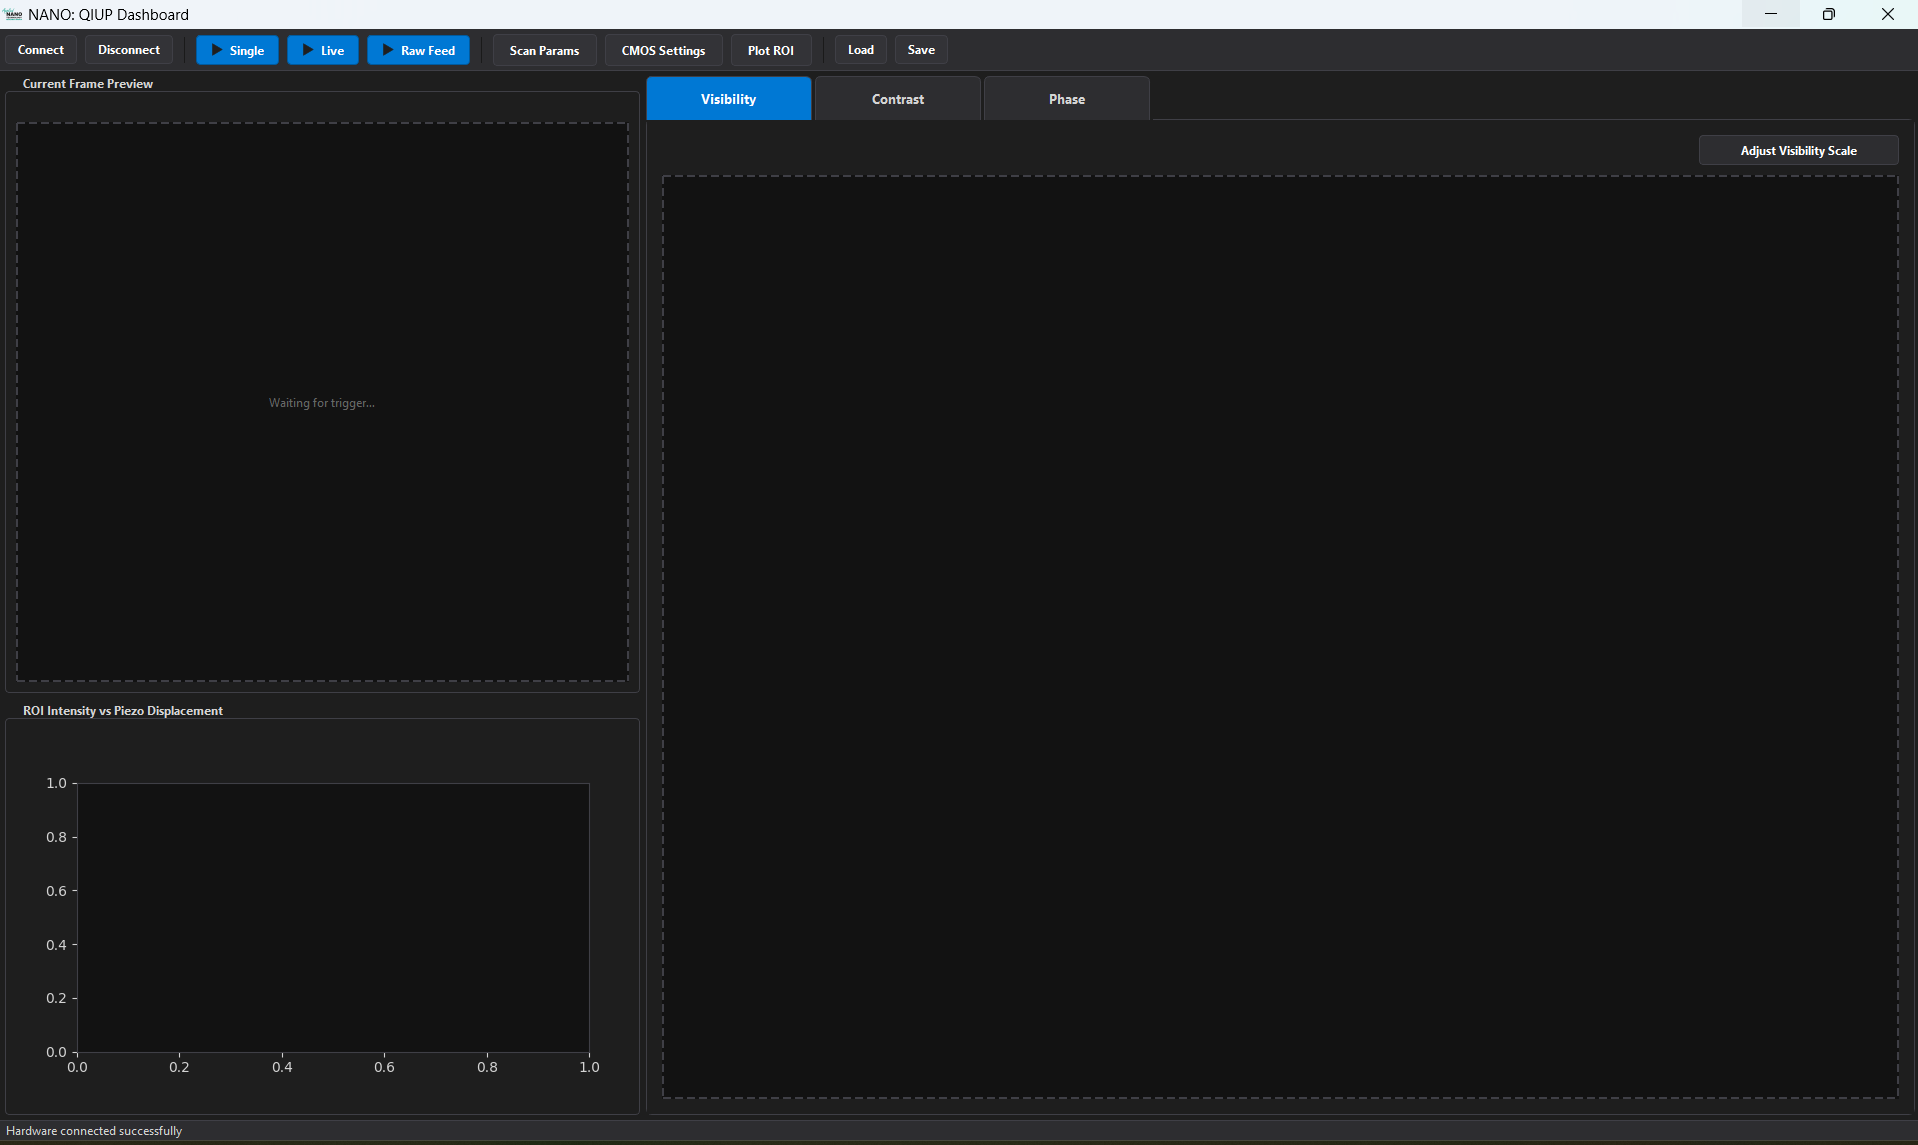
\includegraphics[width=\linewidth]{images/QIUP-tests/Versions/Final_version_app_screenshots/start_screen.png}
            \caption{Layout and design of the custom PyQT5 GUI.}
            \label{fig:gui_layout}
        \end{figure}

        \subsubsection{Real-Time ROI Intensity Monitoring}
        A critical requirement for \ac{QIUP} alignment is verifying that the piezo stage is actively modulating the interference pattern. To visualize this, the software implements a real-time \ac{ROI} intensity monitor.

        This extracted intensity is immediately passed to an embedded Matplotlib canvas. As the piezo stage steps through its cycle, the software plots the recorded hardware displacement on the X-axis and the ROI mean intensity on the Y-axis. The data points are dynamically sorted by absolute displacement before rendering, which guarantees a clean, unbroken sinusoidal line graph representing the physical interference wave, proving to the operator that the system is properly aligned.

        \subsubsection{Dynamic Scaling Controls}
        Depending on the opacity of the sample, the mathematical amplitude of the extracted \ac{FFT} components can fluctuate dramatically. To accommodate this, the \ac{GUI} features dynamic, user-adjustable scaling controls for the colormaps.

        Instead of re-executing the computationally expensive \ac{FFT} every time the user adjusts a contrast slider, the software separates the physics calculations from the visual rendering. The \texttt{CameraController} caches the raw floating-point arrays (\texttt{last\_visibility}, \texttt{last\_contrast}, \texttt{last\_phase}). The \ac{GUI} provides dual-slider widgets mapped from 0 to 1000, representing a 0.0\% to 100.0\% scaling factor. When a slider is moved, the software takes the cached physics data, applies the percentage-based scaling limits, clips the array bounds and applies the OpenCV colormap (\texttt{cv2.applyColorMap}). This architectural separation allows the operator to dynamically fine-tune the visual contrast of the quantum maps with zero computational latency.

    \subsection{User Experience Design}
    This section covers the safeguards and feedback mechanisms integrated into the application to ensure smooth and error-free operation.

        \subsubsection{Workflow Optimization}
        Because the demonstrator is intended to be operated by users with varying levels of technical expertise, the software enforces a strict, linear operational workflow designed to minimize setup errors:
        \begin{enumerate}
            \item \textbf{Connect:} Upon launch, all acquisition controls are disabled. The user must click the "Connect" button, which triggers the hardware initialization.
            \item \textbf{Align:} Once connected, the user utilizes the "Raw Feed" button to stream continuous frames from the \ac{CMOS} sensor, allowing them to manually adjust mirrors and align the sample without triggering the piezo stage.
            \item \textbf{Acquire \& Process:} Following alignment, the user can select "Single" scan or "Live" continuous processing. The software automatically handles the synchronization, \ac{FFT} execution and map rendering.
        \end{enumerate}

        To prevent race conditions or hardware crashes, aggressive input validation is implemented. While an acquisition loop is running, all conflicting controls (such as the disconnect button, manual sliders, or triggering secondary scans) are disabled via \texttt{setEnabled(False)}. Furthermore, destructive actions, such as disconnecting hardware or closing the application, are safeguarded by \texttt{QMessageBox} confirmation dialogs to prevent accidental data loss.

        \subsubsection{Visual Feedback}
        Providing the operator with clear, immediate feedback regarding the system's state is essential for a reliable user experience. The application replaces standard static buttons with dynamic \ac{GUI} elements. For instance, the standard play icons automatically switch to stop icons during live acquisition and the button text updates to "Acquiring..." to indicate active background tasks.

        A dedicated \texttt{QStatusBar} anchors the bottom of the interface, continuously displaying system telemetry. During a scan, it outputs the current frame progress. Upon completion, the \ac{FFT} worker thread calculates the exact execution time via \texttt{time.perf\_counter()} and appends the processing latency to the status bar, proving the system's performance.

        In the event of hardware failure (e.g., a dropped camera frame or a piezo serial timeout), the background worker threads catch the exception and emit an \texttt{error\_signal}. The main \ac{GUI} thread intercepts this signal, safely aborts the active loop, relaxes the piezo crystal and displays a non-blocking warning dialog. This graceful degradation strategy ensures that hardware communication errors do not cause the Python interpreter to crash, allowing the operator to adjust cables or settings and immediately try again.

    \subsection{Design of new Samples}
    To effectively showcase these quantum optical effects to an audience, high-quality, recognizable target samples are required. 

    Because the optical beam diameter in the demonstrator is relatively small, these samples must be fabricated with high spatial precision. New target samples were digitally designed using Adobe Illustrator and manufactured using a laser cutter at the Saxion FabLab. To ensure the laser cutter correctly interpreted the vector paths as through-cuts rather than surface engravings, all cut outlines in the digital files were strictly formatted with a pure magenta stroke color, so the machine is able to determine where to cut \cite{Fablabwiki}.  

    The physical samples were cut from opaque paper. Two distinct shapes were chosen to effectively demonstrate the imaging resolution: a cat silhouette and the Greek letter Psi ($\Psi$). 

    The digital vector designs and their corresponding physical realizations are presented in Figure \ref{fig:sample_fabrication}.

    \begin{figure}[H]
        \centering
        
        % --- Row 1: Vector Designs ---
        \begin{subfigure}[b]{0.45\linewidth}
            \centering
            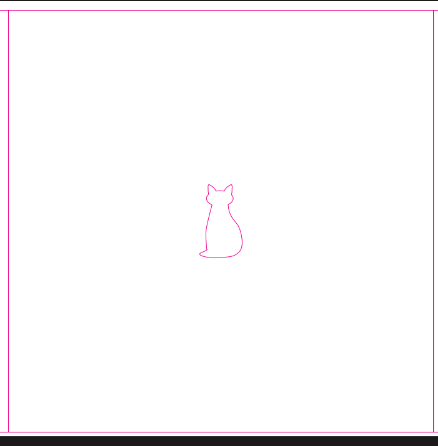
\includegraphics[width=\linewidth]{images/components/samples/cat_cutout.png}
            \caption{Cat vector design (magenta cut path).}
            \label{subfig:cat_design}
        \end{subfigure}
        \hfill % Adds horizontal space between the images
        \begin{subfigure}[b]{0.45\linewidth}
            \centering
            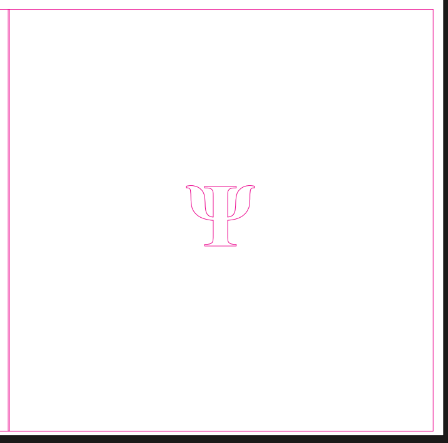
\includegraphics[width=\linewidth]{images/components/samples/psi_cutout.png}
            \caption{Psi vector design (magenta cut path).}
            \label{subfig:psi_design}
        \end{subfigure}
        
        \vspace{0.5cm} % Adds vertical space between the top and bottom rows
        
        % --- Row 2: Physical Samples ---
        \begin{subfigure}[b]{0.45\linewidth}
            \centering
            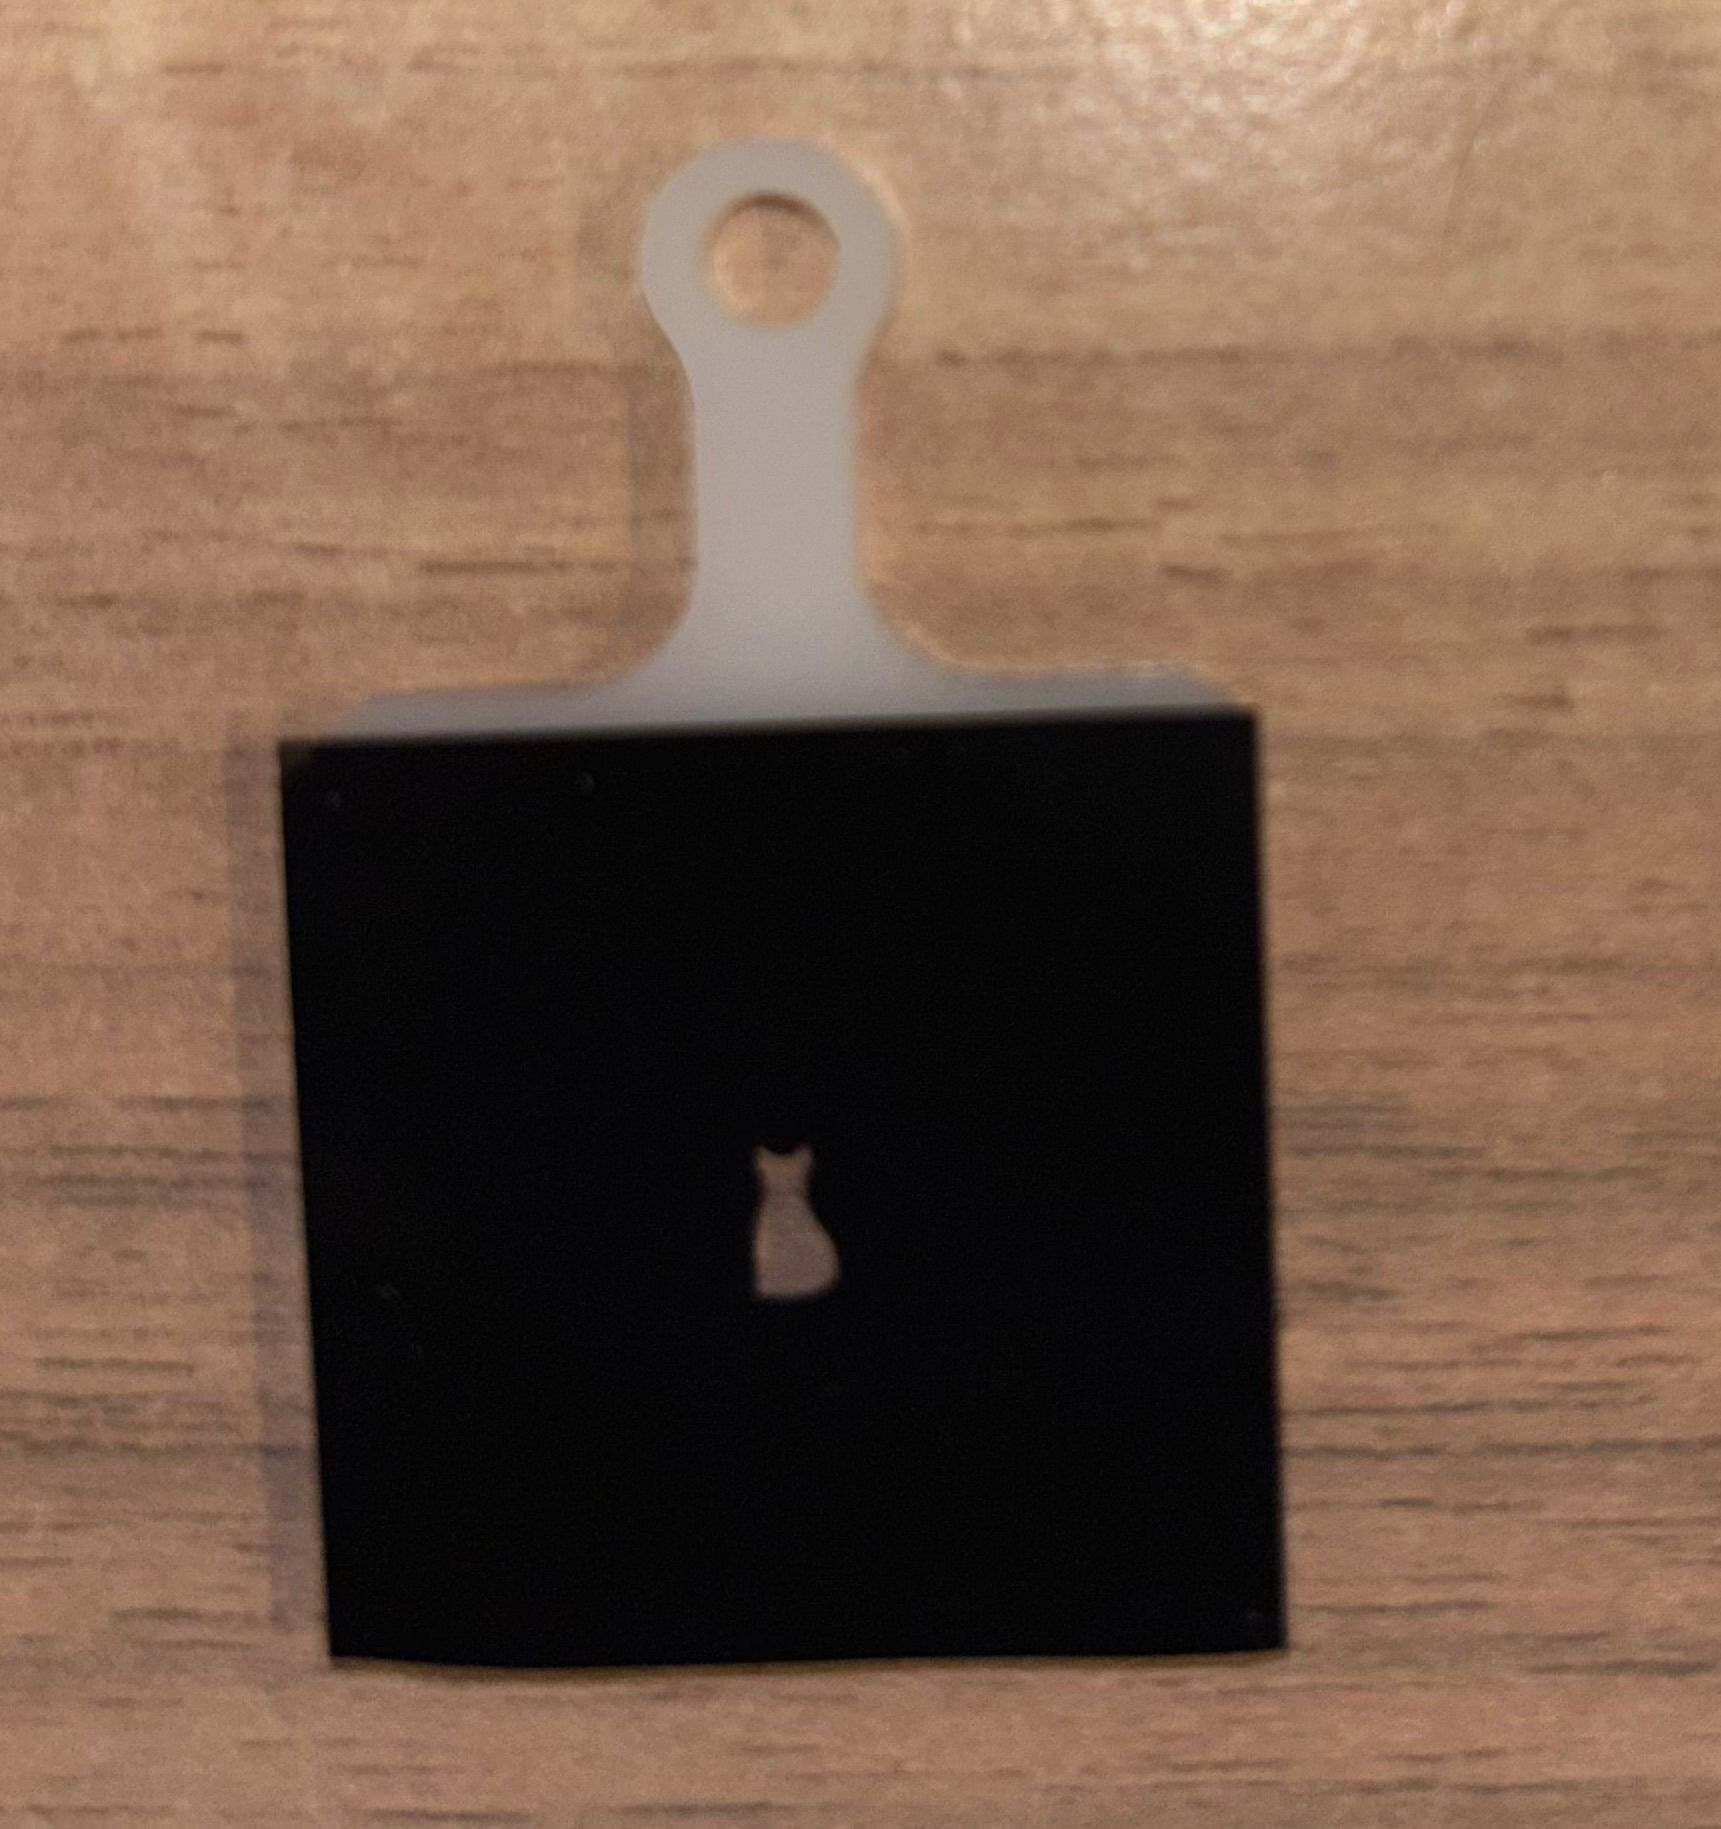
\includegraphics[width=\linewidth]{images/components/samples/Cat.jpeg}
            \caption{Mounted physical cat sample.}
            \label{subfig:cat_sample}
        \end{subfigure}
        \hfill % Adds horizontal space between the images
        \begin{subfigure}[b]{0.45\linewidth}
            \centering
            \includegraphics[width=\linewidth]{images/components/samples/psi.jpeg}
            \caption{Mounted physical Psi sample.}
            \label{subfig:psi_sample}
        \end{subfigure}
        
        % Main Caption and Label
        \caption{Design and cutout of the newly designed samples}
        \label{fig:sample_fabrication}
    \end{figure}

\newpage
\section{Realisation}
This chapter documents the actual execution of the project, including the development sprints, the challenges encountered, and the specific code implementations.

    \subsection{Development Process}
        \subsubsection{Sprint Overview}
            Implementing all necessary hardware control, synchronization and image processing within a single software application required a structured development process. The project was divided into regular one- to two-week sprints, each with technical milestones discussed and planned with the project's supervisor. 
            
            This iterative approach allowed for continuous feedback and incremental progress, as there were no rigid final design specifications at the start of the project, only the general goal of implementing a real-time \ac{QIUP} demonstrator and reconstructing the visibility, contrast, and phase maps.

        \subsubsection{Key Technical Challenges}
            During the realization phase, several significant challenges had to be overcome to achieve a stable, real-time demonstrator:

            \begin{itemize}
                \item \textbf{Kinesis .NET API Bridge and Lack of Documentation:} 
                One of the most time-consuming challenges was integrating the Thorlabs piezoelectric stage and strain gauge. Thorlabs provides some documentation for C/C++ not including the \ac{KPZ101} or \ac{KSG101}, there is a severe lack of official documentation or examples for implementing the Kinesis API in Python. To overcome this, the \texttt{pythonnet} library was used to bridge the \ac{CLR}, but the exact method names and parameters were unknown. The solution involved using Python's built-in \texttt{dir()} introspection function to reverse-engineer the loaded .NET objects in the console. This revealed the available internal methods for both the \ac{KPZ101} and \ac{KSG101} (the full list of discovered methods is provided in Appendix \ref{app:kinesis_dir}). Additionally, translating Python data types into strictly typed C\# formats required explicit casting, such as wrapping Python floats in \texttt{System.Convert.ToDecimal()} to prevent runtime crashes.

                \item \textbf{Piezo Hysteresis and Dual-Mode Control:}
                Initially, the piezo stage was driven in Open-Loop mode by setting raw voltage values. There was a theoretical concern that the inherent hysteresis of the piezoelectric crystal would cause uneven spatial phase steps, potentially degrading the \ac{FFT} output. To address this, the software was expanded to support Closed-Loop control utilizing the reverse-engineered methods found via the \texttt{dir()} command. This required engaging the hardware PID servo via \texttt{SetPositionControlMode} and driving the actuator using \texttt{SetPercentageTravel()}, relying on the KSG101 for exact nanometer-scale readbacks. However, experimental testing revealed that over the short scanning distances required for the demonstrator, the hysteresis was actually not significant, and the quality of the calculated images was practically unaffected. Because open-loop execution completely avoids the settling delay of the hardware PID loop, an Open-Loop version was formally integrated into the final software as well, providing a much faster, highly responsive mode that is ideal for real-time live demonstrations.

                \item \textbf{Camera Buffer Staleness:}
                During early testing of the automated acquisition sequence, the processed interference patterns appeared distorted or completely washed out. Debugging revealed that the \ac{TSI} camera's internal hardware buffer was holding onto "stale" frames. When the software triggered a capture after moving the piezo, it would occasionally retrieve an old frame from before the piezo had settled. This was solved by implementing a strict buffer flush loop immediately before issuing the software trigger, forcefully clearing any pending frames using \texttt{get\_pending\_frame\_or\_null()} to guarantee the next captured image exactly matched the current physical phase step.

                \item \textbf{FFT Performance Bottleneck:}
                The initial image processing pipeline utilized standard \texttt{numpy.fft}. For a $1440 \times 1080$ pixel sensor, processing a 32-frame stack took over a full second, which completely froze the \ac{GUI} and made live demonstration impossible. To solve this, the pipeline was rebuilt using \texttt{pyFFTW}. By implementing pre-allocated, memory-aligned arrays and utilizing \ac{FFTW} plan caching, the execution time was drastically reduced, allowing the system to achieve the low-latency processing required for a smooth user experience.
            \end{itemize}
            
        \subsubsection{Code Organization}
            The software is organized into 6 individual Python scripts, each responsible for a specific aspect of the system's functionality:
            \begin{itemize}
                \item \texttt{main.py}: The entry point of the application, responsible for launching the PyQt5 GUI and initializing the main window.
                \item \texttt{camera\_controller.py}: Contains the \texttt{CameraController} class, which manages all interactions with the Thorlabs Zelux camera, including acquisition control and image processing.
                \item \texttt{camera\_windows\_setup.py}: Handles the setup and configuration of the camera drivers on Windows systems.
                \item \texttt{piezo\_control.py}: Implements the Open -and Closed-Loop control mode for the piezo stage, depending of the applications version, allowing direct voltage control.
                \item \texttt{acquisition\_worker.py}: Contains the \texttt{SingleAcquisitionWorker}, \texttt{LiveProcessingWorker} and \texttt{LiveFeedWorker} classes, which manage the asynchronous acquisition and processing workflows in separate threads.
                \item \texttt{ui\_components.py}: Contains the custom PyQt5 widget classes, such as \texttt{ScalableImageLabel} and \texttt{ClickableLabel}, which provide enhanced functionality for displaying images and handling user interactions.
            \end{itemize}
            A virtual environment has been setup to manage dependencies, using python 3.14, PyQt5 for the \ac{GUI}, pyFFTW for the FFT processing, and the Thorlabs \ac{TSI} \ac{SDK} for camera control. The project structure is designed to maintain a clear separation of concerns, allowing for easier maintenance and future scalability.

    \subsection{Implementation Details}
    This section highlights specific code-level solutions developed to handle piezo control, thread synchronization, and FFT processing.
    
        \subsubsection{Piezo Control Evolution}
            The realization of the piezo control ultimately resulted in two distinct implementations designed to address different use cases. 
            
            The Open-Loop version (\texttt{piezo\_control\_open.py}) prioritizes speed. It drives the actuator by directly mapping the user's target voltage (typically between 0 and 4.5V for one cycle) to the \ac{KPZ101} using \texttt{SetOutputVoltage()}. This mode executes almost instantly but provides no automatic physical verification.
            
            Conversely, the Closed-Loop version (\texttt{piezo\_control\_closed.py}) prioritizes mathematical accuracy. It engages the hardware PID servo via \texttt{SetPositionControlMode(PiezoControlModeTypes.ClosedLoop)}. To bypass specific unit translation errors inherent in the undocumented Kinesis API, it commands the stage using \texttt{SetPercentageTravel()}, calculating the required percentage based on the 20\,$\mu$m maximum travel range. Both versions consistently rely on the KSG101 strain gauge to read the true physical displacement via \texttt{GetReading()}.

        \subsubsection{Acquisition Worker Synchronization}
            To guarantee that every captured frame perfectly matches the intended phase step, a strict synchronization loop is implemented within the \texttt{SingleAcquisitionWorker} thread. The synchronization executes sequentially:
            \begin{enumerate}
                \item Command the piezo stage to move to the next target position.
                \item Call \texttt{time.sleep(settling\_time)} to allow mechanical vibrations to completely dampen.
                \item Flush the camera's internal memory buffer by repeatedly calling \texttt{get\_pending\_frame\_or\_null()} in a \texttt{while} loop until it returns \texttt{None}, destroying any stale frames.
                \item Issue a fresh software trigger via \texttt{issue\_software\_trigger()}.
                \item Retrieve the new, synchronized frame and emit it to the \ac{GUI} thread.
            \end{enumerate}

        \subsubsection{FFT Processing Pipeline}
            The \ac{FFT} pipeline in the \texttt{CameraController} is highly optimized for repetitive live tasks. It implements a specific plan-caching logic: the pyFFTW execution plan (\texttt{self.\_fft\_plan}) is mathematically optimized and built during the first execution. The software only destroys and reconstructs this plan if the user explicitly alters the number of frames (\texttt{n\_frames}) in the \ac{GUI}. 
            
            For rendering, a dynamic range calculation separates the complex physics math from the visual dashboard. The raw, floating-point data maps (Visibility, Contrast, Phase) are held in cache. The GUI sliders provide generic percentage values (0.0 to 100.0\%), which the controller maps to either the theoretical limits (in open loop) or the absolute data limits (e.g., the exact minimum and maximum floats of the current contrast array in closed loop). This separation allows the user to perform real-time colormap contrast adjustments instantly, without recalculating the heavy 1.5-megapixel \ac{FFT}.

        \subsection{UI Design}
            Throughout this internship the Userinterface was iteratively refined based on feedback from the research group and testing sessions. The final design features a modern dark theme with intuitive controls, real-time feedback and dynamic scaling options to accommodate a wide range of sample opacities. The layout is organized to provide clear visual separation between raw hardware telemetry and the processed quantum maps, while custom widgets enhance interactivity and data visualization as shown in Figure \ref{fig:gui_layout}.
            Nonetheless, there have been other design iterations that were tested but ultimately rejected. For instance, an early version of the GUI featured a single unified display for all three quantum maps with toggle buttons to switch between them. However, this was found to be less effective for live demonstrations, as it was required to enlarge the display to show fine details, which made it difficult for the audience to quickly compare the different maps, as illustrated in Figure \ref{fig:gui_layout_v1}.

            \begin{figure}[H]
                \centering
                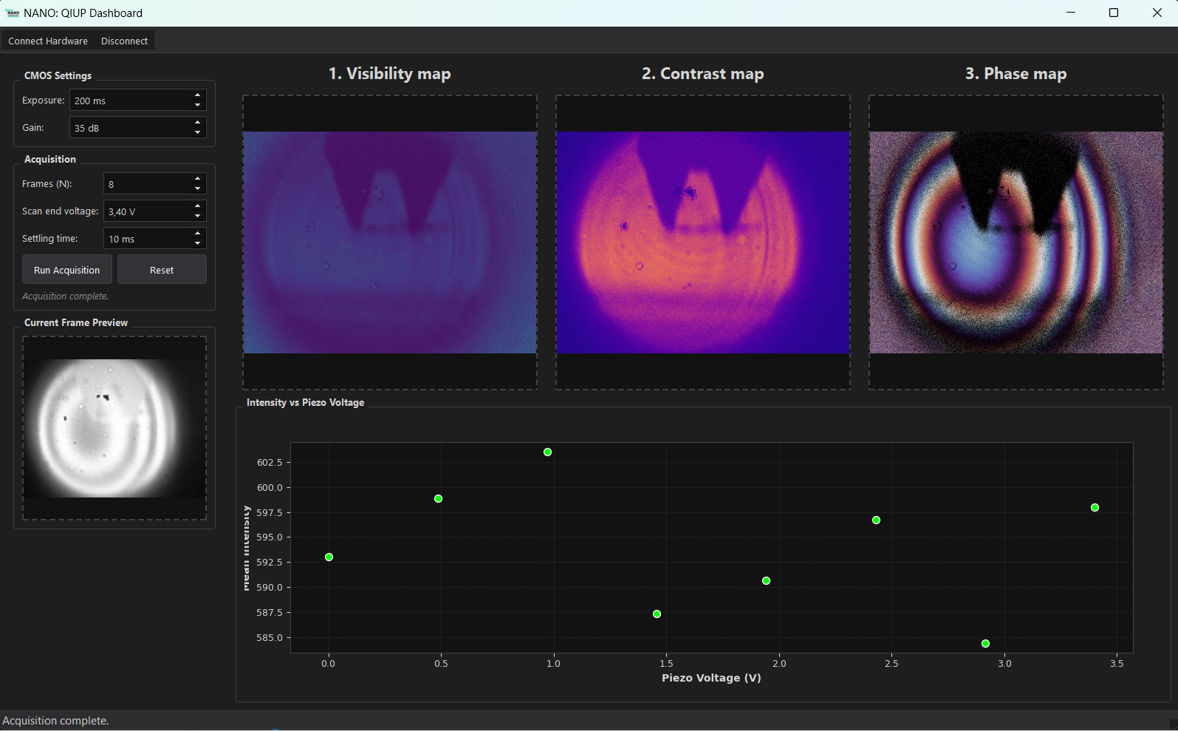
\includegraphics[width=\linewidth]{images/QIUP-tests/Versions/Version1/v1_qiup.png}
                \caption{Layout of the old design and custom PyQT5 GUI.}
                \label{fig:gui_layout_v1}
            \end{figure}

\newpage
\section{Testing}
This chapter details the testing methodologies applied to verify the system's hardware synchronization, processing accuracy, and overall usability.

\subsection{Interference Pattern Validation}
    Before executing the full \ac{FFT}, it is critical to validate that the hardware synchronization correctly captures the underlying quantum interference pattern. To demonstrate this, a high-resolution phase scan was performed using 60 discrete frames to carefully map the sinusoidal intensity oscillation of the signal photons as the piezo stage shifts the optical path length.

    The raw data acquired from the \ac{CMOS} sensor inherently contains high-frequency spatial noise, such as read noise and shot noise, which can disrupt pixel-wise calculations. To mitigate this and improve the \ac{SNR}, the software includes a configurable spatial moving average (MA) filter. Figure \ref{fig:oscillation_comparison} illustrates the direct impact of this filter on the extracted \ac{ROI} intensity using a 3x3 kernel.

    \begin{figure}[H]
        \centering
        % Left plot: Without Filtering
        \begin{subfigure}[b]{0.48\linewidth}
            \centering
            
\includegraphics[width=\linewidth]{"images/QIUP-tests/real representation/without_ma.png"}
            \caption{Sinusoidal oscillation without filtering.}
            \label{fig:real_unfiltered}
        \end{subfigure}
        \hfill % Ensures the images sit side-by-side
        % Right plot: With Filtering
        \begin{subfigure}[b]{0.48\linewidth}
            \centering
            
\includegraphics[width=\linewidth]{"images/QIUP-tests/real representation/with_ma.png"}
            \caption{Sinusoidal oscillation with filtering.}
            \label{fig:real_filtered}
        \end{subfigure}
        
        \caption{Comparative analysis of the interference signal quality, demonstrating the noise reduction achieved through spatial moving average (MA) filtering.}
        \label{fig:oscillation_comparison}
    \end{figure}

    As evident in Figure \ref{fig:real_unfiltered}, the raw intensity curve is more erratic and impacted by sensor noise. Conversely, the filtered data (Figure \ref{fig:real_filtered}) demonstrates a smoother sinusoidal oscillation. This successful extraction confirms two critical system capabilities: first, that the automated hardware synchronization reliably resolves the physical interference pattern, and second, that the spatial moving average filter significantly enhances the \ac{SNR}, providing a highly stabilized data stack for the subsequent \ac{FFT} pipeline.

    \subsection{Piezo Hysteresis Analysis}
    As mentioned earlier in this report, the piezoelectric stage exhibits a hysteresis effect in open-loop mode, meaning the physical displacement of the stage is non-linear with respect to the input voltage. Furthermore, the displacement at a given voltage can vary depending on the settling time. Because the system is designed to be a live demonstrator, this settling time must be kept to a minimum.

    Figure \ref{fig:open_loop_hysteresis_comparison} illustrates this hysteresis behavior across multiple test runs over a voltage range of 0 to 75 V. Each plot displays the relationship between the commanded voltage and the actual displacement measured by the \ac{KSG101}. A distinct hysteresis loop is evident, with the forward voltage sweeps producing different displacements. 

    \begin{figure}[H]
        \centering
        % First plot
        \begin{subfigure}[b]{0.32\linewidth}
            \centering
            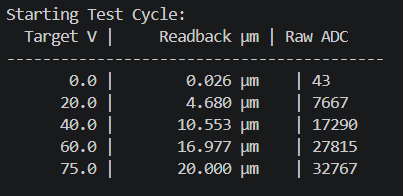
\includegraphics[width=\linewidth]{images/QIUP-tests/Piezo/Open/open_loop_feedback_1.png}
            \caption{Hysteresis test 1}
            \label{subfig:open_loop_75_1}
        \end{subfigure}
        \hfill
        % Second plot
        \begin{subfigure}[b]{0.32\linewidth}
            \centering
            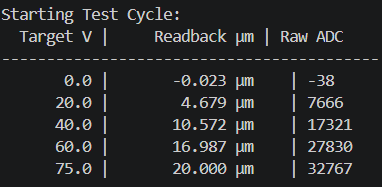
\includegraphics[width=\linewidth]{images/QIUP-tests/Piezo/Open/open_loop_feedback_2.png}
            \caption{Hysteresis test 2}
            \label{subfig:open_loop_75_2}
        \end{subfigure}
        \hfill
        % Third plot
        \begin{subfigure}[b]{0.32\linewidth}
            \centering
            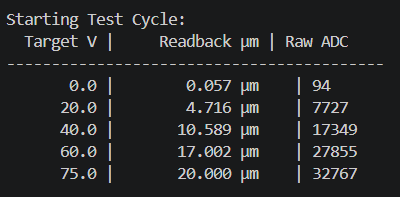
\includegraphics[width=\linewidth]{images/QIUP-tests/Piezo/Open/open_loop_feedback_3.png}
            \caption{Hysteresis test 3}
            \label{subfig:open_loop_75_3}
        \end{subfigure}
        
        \caption{Analysis of open-loop piezoelectric hysteresis across three consecutive test runs (0-75 V), demonstrating the repeatability and characteristics of the actuator.}
        \label{fig:open_loop_hysteresis_comparison}
    \end{figure}

    The translation stage is required to move the sampling mirror by distances corresponding to the signal photon's wavelength of 810 nm. At this scale, the hysteresis effect does not significantly degrade the quality of the calculated images, as the phase steps remain consistent enough to produce clear, oscillating interference patterns within the operational range of approximately 0 to 4.5 V.

    Figure \ref{fig:open_loop_hysteresis_comparison_45} details the hysteresis behavior across multiple test runs specifically within this 0 to 4.5 V operational range used for the demonstrator with 0.5V steps. While a slight hysteresis loop is still observable, the displacement trajectories are much more consistent and closely aligned across the three tests. This indicates that within this narrow operational range, the hysteresis effect is minimal and does not substantially impact overall system performance.

    \begin{figure}[H]
        \centering
        % First plot
        \begin{subfigure}[b]{0.4\linewidth}
            \centering
            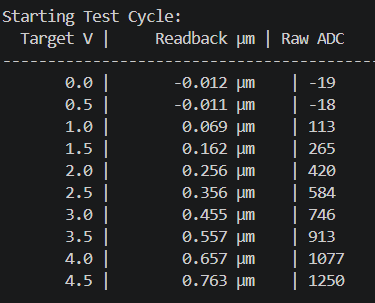
\includegraphics[width=\linewidth]{images/QIUP-tests/Piezo/0to4/open_loop_45_1.png}
            \caption{Hysteresis test 1}
            \label{subfig:open_loop_1}
        \end{subfigure}
        \hfill
        % Second plot
        \begin{subfigure}[b]{0.4\linewidth}
            \centering
            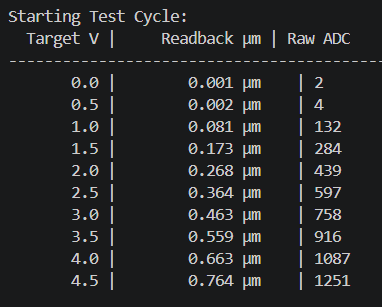
\includegraphics[width=\linewidth]{images/QIUP-tests/Piezo/0to4/open_loop_45_2.png}
            \caption{Hysteresis test 2}
            \label{subfig:open_loop_2}
        \end{subfigure}
        \hfill
        % Third plot
        \begin{subfigure}[b]{0.4\linewidth}
            \centering
            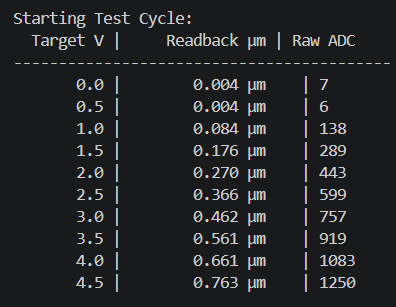
\includegraphics[width=\linewidth]{images/QIUP-tests/Piezo/0to4/open_loop_45_3.png}
            \caption{Hysteresis test 3}
            \label{subfig:open_loop_3}
        \end{subfigure}
        
        \caption{Analysis of open-loop piezoelectric hysteresis across three consecutive test runs (0-4.5 V), demonstrating the repeatability and characteristics of the actuator.}
        \label{fig:open_loop_hysteresis_comparison_45}
    \end{figure}

    \subsection{Open-loop vs. Closed-loop Comparison}
    At the beginning of the project, there was a theoretical concern that the hysteresis of the piezoelectric stage in open-loop mode would cause uneven spatial phase steps. This could potentially degrade the quality of the \ac{FFT} output and, hence the calculated quantum maps. To address this, both open-loop and closed-loop control modes were implemented and tested using the fabricated samples.

        \subsubsection{Open-loop Imaging}
        In open-loop mode, which controls only the target voltage without active position feedback, the system successfully produces clear visibility, contrast, and phase maps of the samples, as shown in Figures \ref{fig:open_loop_cat_noma_grid}, \ref{fig:open_loop_cat_ma_grid}, \ref{fig:open_loop_psi_noma_grid}, and \ref{fig:open_loop_psi_ma_grid}. Overall image quality remains consistent across different frame counts, with the expected increase in noise at lower counts due to reduced averaging. Furthermore, the application of MA yields a distinct improvement in visual quality compared to the non-MA acquisitions, the MA images exhibit noticeably reduced background noise and enhanced contrast, resulting in sharper and more clearly defined features within the final quantum maps.
        \begin{figure}[H] 
            \centering
            
            % ==========================================
            % ROW 1: 3 Frames (No MA)
            % ==========================================
            \begin{subfigure}[b]{0.32\linewidth}
                \centering
                
\includegraphics[width=\linewidth]{"images/QIUP-tests/open loop acquisitions/CAT/no_ma/3_frames_Acquisition_08_06_2026/visibility_map.png"}
                \caption{Visibility (3 frames)}
                \label{subfig:noma_vis_3}
            \end{subfigure}
            \hfill
            \begin{subfigure}[b]{0.32\linewidth}
                \centering
                
\includegraphics[width=\linewidth]{"images/QIUP-tests/open loop acquisitions/CAT/no_ma/3_frames_Acquisition_08_06_2026/contrast_map.png"}
                \caption{Contrast (3 frames)}
                \label{subfig:noma_cont_3}
            \end{subfigure}
            \hfill
            \begin{subfigure}[b]{0.32\linewidth}
                \centering
                
\includegraphics[width=\linewidth]{"images/QIUP-tests/open loop acquisitions/CAT/no_ma/3_frames_Acquisition_08_06_2026/phase_map.png"}
                \caption{Phase (3 frames)}
                \label{subfig:noma_phase_3}
            \end{subfigure}
            
            \vspace{0.3cm} % Vertical spacing between rows

            % ==========================================
            % ROW 2: 8 Frames (No MA)
            % ==========================================
            \begin{subfigure}[b]{0.32\linewidth}
                \centering
                
\includegraphics[width=\linewidth]{"images/QIUP-tests/open loop acquisitions/CAT/no_ma/8_frames_Acquisition_08_06_2026/visibility_map.png"}
                \caption{Visibility (8 frames)}
                \label{subfig:noma_vis_8}
            \end{subfigure}
            \hfill
            \begin{subfigure}[b]{0.32\linewidth}
                \centering
                
\includegraphics[width=\linewidth]{"images/QIUP-tests/open loop acquisitions/CAT/no_ma/8_frames_Acquisition_08_06_2026/contrast_map.png"}
                \caption{Contrast (8 frames)}
                \label{subfig:noma_cont_8}
            \end{subfigure}
            \hfill
            \begin{subfigure}[b]{0.32\linewidth}
                \centering
                
\includegraphics[width=\linewidth]{"images/QIUP-tests/open loop acquisitions/CAT/no_ma/8_frames_Acquisition_08_06_2026/phase_map.png"}
                \caption{Phase (8 frames)}
                \label{subfig:noma_phase_8}
            \end{subfigure}

            \vspace{0.3cm}

            % ==========================================
            % ROW 3: 16 Frames (No MA)
            % ==========================================
            \begin{subfigure}[b]{0.32\linewidth}
                \centering
                
\includegraphics[width=\linewidth]{"images/QIUP-tests/open loop acquisitions/CAT/no_ma/16_frames_Acquisition_08_06_2026/visibility_map.png"}
                \caption{Visibility (16 frames)}
                \label{subfig:noma_vis_16}
            \end{subfigure}
            \hfill
            \begin{subfigure}[b]{0.32\linewidth}
                \centering
                
\includegraphics[width=\linewidth]{"images/QIUP-tests/open loop acquisitions/CAT/no_ma/16_frames_Acquisition_08_06_2026/contrast_map.png"}
                \caption{Contrast (16 frames)}
                \label{subfig:noma_cont_16}
            \end{subfigure}
            \hfill
            \begin{subfigure}[b]{0.32\linewidth}
                \centering
                
\includegraphics[width=\linewidth]{"images/QIUP-tests/open loop acquisitions/CAT/no_ma/16_frames_Acquisition_08_06_2026/phase_map.png"}
                \caption{Phase (16 frames)}
                \label{subfig:noma_phase_16}
            \end{subfigure}

            \vspace{0.3cm}

            % ==========================================
            % ROW 4: 32 Frames (No MA)
            % ==========================================
            \begin{subfigure}[b]{0.32\linewidth}
                \centering
                
\includegraphics[width=\linewidth]{"images/QIUP-tests/open loop acquisitions/CAT/no_ma/32_frames_Acquisition_08_06_2026/visibility_map.png"}
                \caption{Visibility (32 frames)}
                \label{subfig:noma_vis_32}
            \end{subfigure}
            \hfill
            \begin{subfigure}[b]{0.32\linewidth}
                \centering
                
\includegraphics[width=\linewidth]{"images/QIUP-tests/open loop acquisitions/CAT/no_ma/32_frames_Acquisition_08_06_2026/contrast_map.png"}
                \caption{Contrast (32 frames)}
                \label{subfig:noma_cont_32}
            \end{subfigure}
            \hfill
            \begin{subfigure}[b]{0.32\linewidth}
                \centering
                
\includegraphics[width=\linewidth]{"images/QIUP-tests/open loop acquisitions/CAT/no_ma/32_frames_Acquisition_08_06_2026/phase_map.png"}
                \caption{Phase (32 frames)}
                \label{subfig:noma_phase_32}
            \end{subfigure}

            % Main Caption
            \caption{Comparison of Visibility, Contrast, and Phase reconstructions for the CAT sample using an open-loop phase scan \textbf{without} spatial moving average (no MA) filtering. The rows demonstrate the raw effect of increasing the number of phase-shifted frames ($N=3, 8, 16, 32$) on the \ac{FFT} signal-to-noise ratio.}
            \label{fig:open_loop_cat_noma_grid}
        \end{figure}


        \begin{figure}[H] % [p] is recommended here because 12 images will likely take a full page
            \centering
            
            % ==========================================
            % ROW 1: 3 Frames
            % ==========================================
            \begin{subfigure}[b]{0.32\linewidth}
                \centering
                
\includegraphics[width=\linewidth]{"images/QIUP-tests/open loop acquisitions/CAT/ma/3_frames_ma_Acquisition_08_06_2026/visibility_map.png"}
                \caption{Visibility (3 frames)}
                \label{subfig:vis_3}
            \end{subfigure}
            \hfill
            \begin{subfigure}[b]{0.32\linewidth}
                \centering
                
\includegraphics[width=\linewidth]{"images/QIUP-tests/open loop acquisitions/CAT/ma/3_frames_ma_Acquisition_08_06_2026/contrast_map.png"}
                \caption{Contrast (3 frames)}
                \label{subfig:cont_3}
            \end{subfigure}
            \hfill
            \begin{subfigure}[b]{0.32\linewidth}
                \centering
                
\includegraphics[width=\linewidth]{"images/QIUP-tests/open loop acquisitions/CAT/ma/3_frames_ma_Acquisition_08_06_2026/phase_map.png"}
                \caption{Phase (3 frames)}
                \label{subfig:phase_3}
            \end{subfigure}
            
            \vspace{0.3cm} % Vertical spacing between rows

            % ==========================================
            % ROW 2: 8 Frames
            % ==========================================
            \begin{subfigure}[b]{0.32\linewidth}
                \centering
                
\includegraphics[width=\linewidth]{"images/QIUP-tests/open loop acquisitions/CAT/ma/8_frames_ma_Acquisition_08_06_2026/visibility_map.png"}
                \caption{Visibility (8 frames)}
                \label{subfig:vis_8}
            \end{subfigure}
            \hfill
            \begin{subfigure}[b]{0.32\linewidth}
                \centering
                
\includegraphics[width=\linewidth]{"images/QIUP-tests/open loop acquisitions/CAT/ma/8_frames_ma_Acquisition_08_06_2026/contrast_map.png"}
                \caption{Contrast (8 frames)}
                \label{subfig:cont_8}
            \end{subfigure}
            \hfill
            \begin{subfigure}[b]{0.32\linewidth}
                \centering
                
\includegraphics[width=\linewidth]{"images/QIUP-tests/open loop acquisitions/CAT/ma/8_frames_ma_Acquisition_08_06_2026/phase_map.png"}
                \caption{Phase (8 frames)}
                \label{subfig:phase_8}
            \end{subfigure}

            \vspace{0.3cm}

            % ==========================================
            % ROW 3: 16 Frames
            % ==========================================
            \begin{subfigure}[b]{0.32\linewidth}
                \centering
                
\includegraphics[width=\linewidth]{"images/QIUP-tests/open loop acquisitions/CAT/ma/16_frames_ma_Acquisition_08_06_2026/visibility_map.png"}
                \caption{Visibility (16 frames)}
                \label{subfig:vis_16}
            \end{subfigure}
            \hfill
            \begin{subfigure}[b]{0.32\linewidth}
                \centering
                
\includegraphics[width=\linewidth]{"images/QIUP-tests/open loop acquisitions/CAT/ma/16_frames_ma_Acquisition_08_06_2026/contrast_map.png"}
                \caption{Contrast (16 frames)}
                \label{subfig:cont_16}
            \end{subfigure}
            \hfill
            \begin{subfigure}[b]{0.32\linewidth}
                \centering
                
\includegraphics[width=\linewidth]{"images/QIUP-tests/open loop acquisitions/CAT/ma/16_frames_ma_Acquisition_08_06_2026/phase_map.png"}
                \caption{Phase (16 frames)}
                \label{subfig:phase_16}
            \end{subfigure}

            \vspace{0.3cm}

            % ==========================================
            % ROW 4: 32 Frames
            % ==========================================
            \begin{subfigure}[b]{0.32\linewidth}
                \centering
                
\includegraphics[width=\linewidth]{"images/QIUP-tests/open loop acquisitions/CAT/ma/32_frames_ma_Acquisition_08_06_2026/visibility_map.png"}
                \caption{Visibility (32 frames)}
                \label{subfig:vis_32}
            \end{subfigure}
            \hfill
            \begin{subfigure}[b]{0.32\linewidth}
                \centering
                
\includegraphics[width=\linewidth]{"images/QIUP-tests/open loop acquisitions/CAT/ma/32_frames_ma_Acquisition_08_06_2026/contrast_map.png"}
                \caption{Contrast (32 frames)}
                \label{subfig:cont_32}
            \end{subfigure}
            \hfill
            \begin{subfigure}[b]{0.32\linewidth}
                \centering
                
\includegraphics[width=\linewidth]{"images/QIUP-tests/open loop acquisitions/CAT/ma/32_frames_ma_Acquisition_08_06_2026/phase_map.png"}
                \caption{Phase (32 frames)}
                \label{subfig:phase_32}
            \end{subfigure}

            % Main Caption
            \caption{Comparison of Visibility, Contrast, and Phase reconstructions for the CAT sample using an open-loop phase scan with moving average (MA) filtering. The rows demonstrate the effect of increasing the number of phase-shifted frames ($N=3, 8, 16, 32$) on the \ac{FFT} signal-to-noise ratio and image fidelity.}
            \label{fig:open_loop_cat_ma_grid}
        \end{figure}

        \begin{figure}[H] 
            \centering
            
            % ==========================================
            % ROW 1: 3 Frames (No MA)
            % ==========================================
            \begin{subfigure}[b]{0.32\linewidth}
                \centering
                
\includegraphics[width=\linewidth]{"images/QIUP-tests/open loop acquisitions/PSI/no_ma/3_frames_Acquisition_08_06_2026/visibility_map.png"}
                \caption{Visibility (3 frames)}
                \label{subfig:psi_noma_vis_3}
            \end{subfigure}
            \hfill
            \begin{subfigure}[b]{0.32\linewidth}
                \centering
                
\includegraphics[width=\linewidth]{"images/QIUP-tests/open loop acquisitions/PSI/no_ma/3_frames_Acquisition_08_06_2026/contrast_map.png"}
                \caption{Contrast (3 frames)}
                \label{subfig:psi_noma_cont_3}
            \end{subfigure}
            \hfill
            \begin{subfigure}[b]{0.32\linewidth}
                \centering
                
\includegraphics[width=\linewidth]{"images/QIUP-tests/open loop acquisitions/PSI/no_ma/3_frames_Acquisition_08_06_2026/phase_map.png"}
                \caption{Phase (3 frames)}
                \label{subfig:psi_noma_phase_3}
            \end{subfigure}
            
            \vspace{0.3cm} 

            % ==========================================
            % ROW 2: 8 Frames (No MA)
            % ==========================================
            \begin{subfigure}[b]{0.32\linewidth}
                \centering
                
\includegraphics[width=\linewidth]{"images/QIUP-tests/open loop acquisitions/PSI/no_ma/8_frames_Acquisition_08_06_2026/visibility_map.png"}
                \caption{Visibility (8 frames)}
                \label{subfig:psi_noma_vis_8}
            \end{subfigure}
            \hfill
            \begin{subfigure}[b]{0.32\linewidth}
                \centering
                
\includegraphics[width=\linewidth]{"images/QIUP-tests/open loop acquisitions/PSI/no_ma/8_frames_Acquisition_08_06_2026/contrast_map.png"}
                \caption{Contrast (8 frames)}
                \label{subfig:psi_noma_cont_8}
            \end{subfigure}
            \hfill
            \begin{subfigure}[b]{0.32\linewidth}
                \centering
                
\includegraphics[width=\linewidth]{"images/QIUP-tests/open loop acquisitions/PSI/no_ma/8_frames_Acquisition_08_06_2026/phase_map.png"}
                \caption{Phase (8 frames)}
                \label{subfig:psi_noma_phase_8}
            \end{subfigure}

            \vspace{0.3cm}

            % ==========================================
            % ROW 3: 16 Frames (No MA)
            % ==========================================
            \begin{subfigure}[b]{0.32\linewidth}
                \centering
                
\includegraphics[width=\linewidth]{"images/QIUP-tests/open loop acquisitions/PSI/no_ma/16_frames_Acquisition_08_06_2026/visibility_map.png"}
                \caption{Visibility (16 frames)}
                \label{subfig:psi_noma_vis_16}
            \end{subfigure}
            \hfill
            \begin{subfigure}[b]{0.32\linewidth}
                \centering
                
\includegraphics[width=\linewidth]{"images/QIUP-tests/open loop acquisitions/PSI/no_ma/16_frames_Acquisition_08_06_2026/contrast_map.png"}
                \caption{Contrast (16 frames)}
                \label{subfig:psi_noma_cont_16}
            \end{subfigure}
            \hfill
            \begin{subfigure}[b]{0.32\linewidth}
                \centering
                
\includegraphics[width=\linewidth]{"images/QIUP-tests/open loop acquisitions/PSI/no_ma/16_frames_Acquisition_08_06_2026/phase_map.png"}
                \caption{Phase (16 frames)}
                \label{subfig:psi_noma_phase_16}
            \end{subfigure}

            \vspace{0.3cm}

            % ==========================================
            % ROW 4: 32 Frames (No MA)
            % ==========================================
            \begin{subfigure}[b]{0.32\linewidth}
                \centering
                
\includegraphics[width=\linewidth]{"images/QIUP-tests/open loop acquisitions/PSI/no_ma/32_frames_Acquisition_08_06_2026/visibility_map.png"}
                \caption{Visibility (32 frames)}
                \label{subfig:psi_noma_vis_32}
            \end{subfigure}
            \hfill
            \begin{subfigure}[b]{0.32\linewidth}
                \centering
                
\includegraphics[width=\linewidth]{"images/QIUP-tests/open loop acquisitions/PSI/no_ma/32_frames_Acquisition_08_06_2026/contrast_map.png"}
                \caption{Contrast (32 frames)}
                \label{subfig:psi_noma_cont_32}
            \end{subfigure}
            \hfill
            \begin{subfigure}[b]{0.32\linewidth}
                \centering
                
\includegraphics[width=\linewidth]{"images/QIUP-tests/open loop acquisitions/PSI/no_ma/32_frames_Acquisition_08_06_2026/phase_map.png"}
                \caption{Phase (32 frames)}
                \label{subfig:psi_noma_phase_32}
            \end{subfigure}

            % Main Caption
            \caption{Comparison of Visibility, Contrast, and Phase reconstructions for the PSI sample using an open-loop phase scan \textbf{without} spatial moving average (no MA) filtering. The rows demonstrate the raw effect of increasing the number of phase-shifted frames ($N=3, 8, 16, 32$) on the \ac{FFT} signal-to-noise ratio.}
            \label{fig:open_loop_psi_noma_grid}
        \end{figure}

        \begin{figure}[H] 
            \centering
            
            % ==========================================
            % ROW 1: 3 Frames (MA)
            % ==========================================
            \begin{subfigure}[b]{0.32\linewidth}
                \centering
                
\includegraphics[width=\linewidth]{"images/QIUP-tests/open loop acquisitions/PSI/ma/3_frames_ma_Acquisition_08_06_2026/visibility_map.png"}
                \caption{Visibility (3 frames)}
                \label{subfig:psi_ma_vis_3}
            \end{subfigure}
            \hfill
            \begin{subfigure}[b]{0.32\linewidth}
                \centering
                
\includegraphics[width=\linewidth]{"images/QIUP-tests/open loop acquisitions/PSI/ma/3_frames_ma_Acquisition_08_06_2026/contrast_map.png"}
                \caption{Contrast (3 frames)}
                \label{subfig:psi_ma_cont_3}
            \end{subfigure}
            \hfill
            \begin{subfigure}[b]{0.32\linewidth}
                \centering
                
\includegraphics[width=\linewidth]{"images/QIUP-tests/open loop acquisitions/PSI/ma/3_frames_ma_Acquisition_08_06_2026/phase_map.png"}
                \caption{Phase (3 frames)}
                \label{subfig:psi_ma_phase_3}
            \end{subfigure}
            
            \vspace{0.3cm}

            % ==========================================
            % ROW 2: 8 Frames (MA)
            % ==========================================
            \begin{subfigure}[b]{0.32\linewidth}
                \centering
                
\includegraphics[width=\linewidth]{"images/QIUP-tests/open loop acquisitions/PSI/ma/8_frames_ma_Acquisition_08_06_2026/visibility_map.png"}
                \caption{Visibility (8 frames)}
                \label{subfig:psi_ma_vis_8}
            \end{subfigure}
            \hfill
            \begin{subfigure}[b]{0.32\linewidth}
                \centering
                
\includegraphics[width=\linewidth]{"images/QIUP-tests/open loop acquisitions/PSI/ma/8_frames_ma_Acquisition_08_06_2026/contrast_map.png"}
                \caption{Contrast (8 frames)}
                \label{subfig:psi_ma_cont_8}
            \end{subfigure}
            \hfill
            \begin{subfigure}[b]{0.32\linewidth}
                \centering
                
\includegraphics[width=\linewidth]{"images/QIUP-tests/open loop acquisitions/PSI/ma/8_frames_ma_Acquisition_08_06_2026/phase_map.png"}
                \caption{Phase (8 frames)}
                \label{subfig:psi_ma_phase_8}
            \end{subfigure}

            \vspace{0.3cm}

            % ==========================================
            % ROW 3: 16 Frames (MA)
            % ==========================================
            \begin{subfigure}[b]{0.32\linewidth}
                \centering
                
\includegraphics[width=\linewidth]{"images/QIUP-tests/open loop acquisitions/PSI/ma/16_frames_ma_Acquisition_08_06_2026/visibility_map.png"}
                \caption{Visibility (16 frames)}
                \label{subfig:psi_ma_vis_16}
            \end{subfigure}
            \hfill
            \begin{subfigure}[b]{0.32\linewidth}
                \centering
                
\includegraphics[width=\linewidth]{"images/QIUP-tests/open loop acquisitions/PSI/ma/16_frames_ma_Acquisition_08_06_2026/contrast_map.png"}
                \caption{Contrast (16 frames)}
                \label{subfig:psi_ma_cont_16}
            \end{subfigure}
            \hfill
            \begin{subfigure}[b]{0.32\linewidth}
                \centering
                
\includegraphics[width=\linewidth]{"images/QIUP-tests/open loop acquisitions/PSI/ma/16_frames_ma_Acquisition_08_06_2026/phase_map.png"}
                \caption{Phase (16 frames)}
                \label{subfig:psi_ma_phase_16}
            \end{subfigure}

            \vspace{0.3cm}

            % ==========================================
            % ROW 4: 32 Frames (MA)
            % ==========================================
            \begin{subfigure}[b]{0.32\linewidth}
                \centering
                
\includegraphics[width=\linewidth]{"images/QIUP-tests/open loop acquisitions/PSI/ma/32_frames_ma_Acquisition_08_06_2026/visibility_map.png"}
                \caption{Visibility (32 frames)}
                \label{subfig:psi_ma_vis_32}
            \end{subfigure}
            \hfill
            \begin{subfigure}[b]{0.32\linewidth}
                \centering
                
\includegraphics[width=\linewidth]{"images/QIUP-tests/open loop acquisitions/PSI/ma/32_frames_ma_Acquisition_08_06_2026/contrast_map.png"}
                \caption{Contrast (32 frames)}
                \label{subfig:psi_ma_cont_32}
            \end{subfigure}
            \hfill
            \begin{subfigure}[b]{0.32\linewidth}
                \centering
                
\includegraphics[width=\linewidth]{"images/QIUP-tests/open loop acquisitions/PSI/ma/32_frames_ma_Acquisition_08_06_2026/phase_map.png"}
                \caption{Phase (32 frames)}
                \label{subfig:psi_ma_phase_32}
            \end{subfigure}

            % Main Caption
            \caption{Comparison of Visibility, Contrast, and Phase reconstructions for the PSI sample using an open-loop phase scan with moving average (MA) filtering. The rows demonstrate the effect of increasing the number of phase-shifted frames ($N=3, 8, 16, 32$) on the \ac{FFT} signal-to-noise ratio and image fidelity.}
            \label{fig:open_loop_psi_ma_grid}
        \end{figure}
        As observed in the acquired maps, the open-loop control mode successfully produces high-fidelity quantum images, clearly resolving visibility, contrast, and phase, despite the inherent hysteresis of the piezoelectric crystal. The reconstructions remain remarkably consistent across varying frame counts, and the application of the spatial moving average (MA) filter yields a significant enhancement in overall clarity. Crucially, the system's robustness against non-linear phase steps is enabled by the dynamic $F_1$ bin auto-detection algorithm detailed earlier. By computationally isolating the dominant interference frequency rather than relying on a strictly defined Fourier bin, the software effectively compensates for slight positional variations during the sweep. This algorithmic resilience actively mitigates spectral leakage, ensuring that the theoretical drawbacks of open-loop hysteresis do not practically degrade the final quantum measurements.

        \subsubsection{Closed-loop imaging}
        In contrast to the open-loop approach, closed-loop imaging actively engages the hardware PID servo and utilizes the strain gauge feedback to guarantee strictly equidistant spatial phase steps. The reconstructed visibility, contrast, and phase maps for this mode are presented in Figures \ref{fig:closed_loop_cat_noma_grid}, \ref{fig:closed_loop_cat_ma_grid}, \ref{fig:closed_loop_psi_noma_grid}, and \ref{fig:closed_loop_psi_ma_grid}. As observed in the open-loop tests, increasing the acquisition frame count progressively enhances the signal-to-noise ratio, and the application of the spatial moving average (MA) filter significantly minimizes background artifacts to yield highly defined edges. While the visual differences between the open-loop and closed-loop maps may appear subtle to the naked eye—validating that piezoelectric hysteresis is minimal over short scanning distances—the closed-loop method fundamentally ensures mathematical accuracy by preventing spectral leakage during the \ac{FFT}. Therefore, while open-loop control remains ideal for rapid live demonstrations, the closed-loop architecture provides the highest fidelity and reliability for quantitative scientific analysis.        

        \begin{figure}[H] 
            \centering
            % ROW 1: 3 Frames (No MA)
            \begin{subfigure}[b]{0.32\linewidth}
                \centering
                
\includegraphics[width=\linewidth]{"images/QIUP-tests/closed loop Acquisitions/CAT/no_ma/3_frames_Acquisition_08_06_2026/visibility_map.png"}
                \caption{Visibility (3 frames)}
            \end{subfigure}
            \hfill
            \begin{subfigure}[b]{0.32\linewidth}
                \centering
                
\includegraphics[width=\linewidth]{"images/QIUP-tests/closed loop Acquisitions/CAT/no_ma/3_frames_Acquisition_08_06_2026/contrast_map.png"}
                \caption{Contrast (3 frames)}
            \end{subfigure}
            \hfill
            \begin{subfigure}[b]{0.32\linewidth}
                \centering
                
\includegraphics[width=\linewidth]{"images/QIUP-tests/closed loop Acquisitions/CAT/no_ma/3_frames_Acquisition_08_06_2026/phase_map.png"}
                \caption{Phase (3 frames)}
            \end{subfigure}
            
            \vspace{0.3cm} 
            % ROW 2: 8 Frames (No MA)
            \begin{subfigure}[b]{0.32\linewidth}
                \centering
                
\includegraphics[width=\linewidth]{"images/QIUP-tests/closed loop Acquisitions/CAT/no_ma/8_frames_Acquisition_08_06_2026/visibility_map.png"}
                \caption{Visibility (8 frames)}
            \end{subfigure}
            \hfill
            \begin{subfigure}[b]{0.32\linewidth}
                \centering
                
\includegraphics[width=\linewidth]{"images/QIUP-tests/closed loop Acquisitions/CAT/no_ma/8_frames_Acquisition_08_06_2026/contrast_map.png"}
                \caption{Contrast (8 frames)}
            \end{subfigure}
            \hfill
            \begin{subfigure}[b]{0.32\linewidth}
                \centering
                
\includegraphics[width=\linewidth]{"images/QIUP-tests/closed loop Acquisitions/CAT/no_ma/8_frames_Acquisition_08_06_2026/phase_map.png"}
                \caption{Phase (8 frames)}
            \end{subfigure}

            \vspace{0.3cm}
            % ROW 3: 16 Frames (No MA)
            \begin{subfigure}[b]{0.32\linewidth}
                \centering
                
\includegraphics[width=\linewidth]{"images/QIUP-tests/closed loop Acquisitions/CAT/no_ma/16_frames_Acquisition_08_06_2026/visibility_map.png"}
                \caption{Visibility (16 frames)}
            \end{subfigure}
            \hfill
            \begin{subfigure}[b]{0.32\linewidth}
                \centering
                
\includegraphics[width=\linewidth]{"images/QIUP-tests/closed loop Acquisitions/CAT/no_ma/16_frames_Acquisition_08_06_2026/contrast_map.png"}
                \caption{Contrast (16 frames)}
            \end{subfigure}
            \hfill
            \begin{subfigure}[b]{0.32\linewidth}
                \centering
                
\includegraphics[width=\linewidth]{"images/QIUP-tests/closed loop Acquisitions/CAT/no_ma/16_frames_Acquisition_08_06_2026/phase_map.png"}
                \caption{Phase (16 frames)}
            \end{subfigure}

            \vspace{0.3cm}
            % ROW 4: 32 Frames (No MA)
            \begin{subfigure}[b]{0.32\linewidth}
                \centering
                
\includegraphics[width=\linewidth]{"images/QIUP-tests/closed loop Acquisitions/CAT/no_ma/32_frames_Acquisition_08_06_2026/visibility_map.png"}
                \caption{Visibility (32 frames)}
            \end{subfigure}
            \hfill
            \begin{subfigure}[b]{0.32\linewidth}
                \centering
                
\includegraphics[width=\linewidth]{"images/QIUP-tests/closed loop Acquisitions/CAT/no_ma/32_frames_Acquisition_08_06_2026/contrast_map.png"}
                \caption{Contrast (32 frames)}
            \end{subfigure}
            \hfill
            \begin{subfigure}[b]{0.32\linewidth}
                \centering
                
\includegraphics[width=\linewidth]{"images/QIUP-tests/closed loop Acquisitions/CAT/no_ma/32_frames_Acquisition_08_06_2026/phase_map.png"}
                \caption{Phase (32 frames)}
            \end{subfigure}

            \caption{CAT sample: Closed-loop phase scan \textbf{without} spatial moving average (no MA) filtering ($N=3, 8, 16, 32$).}
            \label{fig:closed_loop_cat_noma_grid}
        \end{figure}

        \begin{figure}[H] 
            \centering
            % ROW 1: 3 Frames (MA)
            \begin{subfigure}[b]{0.32\linewidth}
                \centering
                
\includegraphics[width=\linewidth]{"images/QIUP-tests/closed loop Acquisitions/CAT/ma/3_frames_ma_Acquisition_08_06_2026/visibility_map.png"}
                \caption{Visibility (3 frames)}
            \end{subfigure}
            \hfill
            \begin{subfigure}[b]{0.32\linewidth}
                \centering
                
\includegraphics[width=\linewidth]{"images/QIUP-tests/closed loop Acquisitions/CAT/ma/3_frames_ma_Acquisition_08_06_2026/contrast_map.png"}
                \caption{Contrast (3 frames)}
            \end{subfigure}
            \hfill
            \begin{subfigure}[b]{0.32\linewidth}
                \centering
                
\includegraphics[width=\linewidth]{"images/QIUP-tests/closed loop Acquisitions/CAT/ma/3_frames_ma_Acquisition_08_06_2026/phase_map.png"}
                \caption{Phase (3 frames)}
            \end{subfigure}
            
            \vspace{0.3cm}
            % ROW 2: 8 Frames (MA)
            \begin{subfigure}[b]{0.32\linewidth}
                \centering
                
\includegraphics[width=\linewidth]{"images/QIUP-tests/closed loop Acquisitions/CAT/ma/8_frames_ma_Acquisition_08_06_2026/visibility_map.png"}
                \caption{Visibility (8 frames)}
            \end{subfigure}
            \hfill
            \begin{subfigure}[b]{0.32\linewidth}
                \centering
                
\includegraphics[width=\linewidth]{"images/QIUP-tests/closed loop Acquisitions/CAT/ma/8_frames_ma_Acquisition_08_06_2026/contrast_map.png"}
                \caption{Contrast (8 frames)}
            \end{subfigure}
            \hfill
            \begin{subfigure}[b]{0.32\linewidth}
                \centering
                
\includegraphics[width=\linewidth]{"images/QIUP-tests/closed loop Acquisitions/CAT/ma/8_frames_ma_Acquisition_08_06_2026/phase_map.png"}
                \caption{Phase (8 frames)}
            \end{subfigure}

            \vspace{0.3cm}
            % ROW 3: 16 Frames (MA)
            \begin{subfigure}[b]{0.32\linewidth}
                \centering
                
\includegraphics[width=\linewidth]{"images/QIUP-tests/closed loop Acquisitions/CAT/ma/16_frames_ma_Acquisition_08_06_2026/visibility_map.png"}
                \caption{Visibility (16 frames)}
            \end{subfigure}
            \hfill
            \begin{subfigure}[b]{0.32\linewidth}
                \centering
                
\includegraphics[width=\linewidth]{"images/QIUP-tests/closed loop Acquisitions/CAT/ma/16_frames_ma_Acquisition_08_06_2026/contrast_map.png"}
                \caption{Contrast (16 frames)}
            \end{subfigure}
            \hfill
            \begin{subfigure}[b]{0.32\linewidth}
                \centering
                
\includegraphics[width=\linewidth]{"images/QIUP-tests/closed loop Acquisitions/CAT/ma/16_frames_ma_Acquisition_08_06_2026/phase_map.png"}
                \caption{Phase (16 frames)}
            \end{subfigure}

            \vspace{0.3cm}
            % ROW 4: 32 Frames (MA)
            \begin{subfigure}[b]{0.32\linewidth}
                \centering
                
\includegraphics[width=\linewidth]{"images/QIUP-tests/closed loop Acquisitions/CAT/ma/32_frames_ma_Acquisition_08_06_2026/visibility_map.png"}
                \caption{Visibility (32 frames)}
            \end{subfigure}
            \hfill
            \begin{subfigure}[b]{0.32\linewidth}
                \centering
                
\includegraphics[width=\linewidth]{"images/QIUP-tests/closed loop Acquisitions/CAT/ma/32_frames_ma_Acquisition_08_06_2026/contrast_map.png"}
                \caption{Contrast (32 frames)}
            \end{subfigure}
            \hfill
            \begin{subfigure}[b]{0.32\linewidth}
                \centering
                
\includegraphics[width=\linewidth]{"images/QIUP-tests/closed loop Acquisitions/CAT/ma/32_frames_ma_Acquisition_08_06_2026/phase_map.png"}
                \caption{Phase (32 frames)}
            \end{subfigure}

            \caption{CAT sample: Closed-loop phase scan with moving average (MA) filtering ($N=3, 8, 16, 32$).}
            \label{fig:closed_loop_cat_ma_grid}
    \end{figure}

    %%%%%%%%%%%%%%%%%%%%%%%%%%%%%%%%%%%%%%%%%%%%%%%%%%%%%%%%%%%%%%%%%%%%%
    \begin{figure}[p] 
        \centering
        % ROW 1: 3 Frames (No MA)
        \begin{subfigure}[b]{0.32\linewidth}
            \centering
            
\includegraphics[width=\linewidth]{"images/QIUP-tests/closed loop Acquisitions/PSI/no_ma/3_frames_Acquisition_08_06_2026/visibility_map.png"}
            \caption{Visibility (3 frames)}
        \end{subfigure}
        \hfill
        \begin{subfigure}[b]{0.32\linewidth}
            \centering
            
\includegraphics[width=\linewidth]{"images/QIUP-tests/closed loop Acquisitions/PSI/no_ma/3_frames_Acquisition_08_06_2026/contrast_map.png"}
            \caption{Contrast (3 frames)}
        \end{subfigure}
        \hfill
        \begin{subfigure}[b]{0.32\linewidth}
            \centering
            
\includegraphics[width=\linewidth]{"images/QIUP-tests/closed loop Acquisitions/PSI/no_ma/3_frames_Acquisition_08_06_2026/phase_map.png"}
            \caption{Phase (3 frames)}
        \end{subfigure}
        
        \vspace{0.3cm} 
        % ROW 2: 8 Frames (No MA)
        \begin{subfigure}[b]{0.32\linewidth}
            \centering
            
\includegraphics[width=\linewidth]{"images/QIUP-tests/closed loop Acquisitions/PSI/no_ma/8_frames_Acquisition_08_06_2026/visibility_map.png"}
            \caption{Visibility (8 frames)}
        \end{subfigure}
        \hfill
        \begin{subfigure}[b]{0.32\linewidth}
            \centering
            
\includegraphics[width=\linewidth]{"images/QIUP-tests/closed loop Acquisitions/PSI/no_ma/8_frames_Acquisition_08_06_2026/contrast_map.png"}
            \caption{Contrast (8 frames)}
        \end{subfigure}
        \hfill
        \begin{subfigure}[b]{0.32\linewidth}
            \centering
            
\includegraphics[width=\linewidth]{"images/QIUP-tests/closed loop Acquisitions/PSI/no_ma/8_frames_Acquisition_08_06_2026/phase_map.png"}
            \caption{Phase (8 frames)}
        \end{subfigure}

        \vspace{0.3cm}
        % ROW 3: 16 Frames (No MA)
        \begin{subfigure}[b]{0.32\linewidth}
            \centering
            
\includegraphics[width=\linewidth]{"images/QIUP-tests/closed loop Acquisitions/PSI/no_ma/16_frames_Acquisition_08_06_2026/visibility_map.png"}
            \caption{Visibility (16 frames)}
        \end{subfigure}
        \hfill
        \begin{subfigure}[b]{0.32\linewidth}
            \centering
            
\includegraphics[width=\linewidth]{"images/QIUP-tests/closed loop Acquisitions/PSI/no_ma/16_frames_Acquisition_08_06_2026/contrast_map.png"}
            \caption{Contrast (16 frames)}
        \end{subfigure}
        \hfill
        \begin{subfigure}[b]{0.32\linewidth}
            \centering
            
\includegraphics[width=\linewidth]{"images/QIUP-tests/closed loop Acquisitions/PSI/no_ma/16_frames_Acquisition_08_06_2026/phase_map.png"}
            \caption{Phase (16 frames)}
        \end{subfigure}

        \vspace{0.3cm}
        % ROW 4: 32 Frames (No MA)
        \begin{subfigure}[b]{0.32\linewidth}
            \centering
            
\includegraphics[width=\linewidth]{"images/QIUP-tests/closed loop Acquisitions/PSI/no_ma/32_frames_Acquisition_08_06_2026/visibility_map.png"}
            \caption{Visibility (32 frames)}
        \end{subfigure}
        \hfill
        \begin{subfigure}[b]{0.32\linewidth}
            \centering
            
\includegraphics[width=\linewidth]{"images/QIUP-tests/closed loop Acquisitions/PSI/no_ma/32_frames_Acquisition_08_06_2026/contrast_map.png"}
            \caption{Contrast (32 frames)}
        \end{subfigure}
        \hfill
        \begin{subfigure}[b]{0.32\linewidth}
            \centering
            
\includegraphics[width=\linewidth]{"images/QIUP-tests/closed loop Acquisitions/PSI/no_ma/32_frames_Acquisition_08_06_2026/phase_map.png"}
            \caption{Phase (32 frames)}
        \end{subfigure}

        \caption{PSI sample: Closed-loop phase scan \textbf{without} spatial moving average (no MA) filtering ($N=3, 8, 16, 32$).}
        \label{fig:closed_loop_psi_noma_grid}
    \end{figure}

    %%%%%%%%%%%%%%%%%%%%%%%%%%%%%%%%%%%%%%%%%%%%%%%%%%%%%%%%%%%%%%%%%%%%%%

    \begin{figure}[p] 
        \centering
        % ROW 1: 3 Frames (MA)
        \begin{subfigure}[b]{0.32\linewidth}
            \centering
            
\includegraphics[width=\linewidth]{"images/QIUP-tests/closed loop Acquisitions/PSI/ma/3_frames_ma_Acquisition_08_06_2026/visibility_map.png"}
            \caption{Visibility (3 frames)}
        \end{subfigure}
        \hfill
        \begin{subfigure}[b]{0.32\linewidth}
            \centering
            
\includegraphics[width=\linewidth]{"images/QIUP-tests/closed loop Acquisitions/PSI/ma/3_frames_ma_Acquisition_08_06_2026/contrast_map.png"}
            \caption{Contrast (3 frames)}
        \end{subfigure}
        \hfill
        \begin{subfigure}[b]{0.32\linewidth}
            \centering
            
\includegraphics[width=\linewidth]{"images/QIUP-tests/closed loop Acquisitions/PSI/ma/3_frames_ma_Acquisition_08_06_2026/phase_map.png"}
            \caption{Phase (3 frames)}
        \end{subfigure}
        
        \vspace{0.3cm}
        % ROW 2: 8 Frames (MA)
        \begin{subfigure}[b]{0.32\linewidth}
            \centering
            
\includegraphics[width=\linewidth]{"images/QIUP-tests/closed loop Acquisitions/PSI/ma/8_frames_ma_Acquisition_08_06_2026/visibility_map.png"}
            \caption{Visibility (8 frames)}
        \end{subfigure}
        \hfill
        \begin{subfigure}[b]{0.32\linewidth}
            \centering
            
\includegraphics[width=\linewidth]{"images/QIUP-tests/closed loop Acquisitions/PSI/ma/8_frames_ma_Acquisition_08_06_2026/contrast_map.png"}
            \caption{Contrast (8 frames)}
        \end{subfigure}
        \hfill
        \begin{subfigure}[b]{0.32\linewidth}
            \centering
            
\includegraphics[width=\linewidth]{"images/QIUP-tests/closed loop Acquisitions/PSI/ma/8_frames_ma_Acquisition_08_06_2026/phase_map.png"}
            \caption{Phase (8 frames)}
        \end{subfigure}

        \vspace{0.3cm}
        % ROW 3: 16 Frames (MA)
        \begin{subfigure}[b]{0.32\linewidth}
            \centering
            
\includegraphics[width=\linewidth]{"images/QIUP-tests/closed loop Acquisitions/PSI/ma/16_frames_ma_Acquisition_08_06_2026/visibility_map.png"}
            \caption{Visibility (16 frames)}
        \end{subfigure}
        \hfill
        \begin{subfigure}[b]{0.32\linewidth}
            \centering
            
\includegraphics[width=\linewidth]{"images/QIUP-tests/closed loop Acquisitions/PSI/ma/16_frames_ma_Acquisition_08_06_2026/contrast_map.png"}
            \caption{Contrast (16 frames)}
        \end{subfigure}
        \hfill
        \begin{subfigure}[b]{0.32\linewidth}
            \centering
            
\includegraphics[width=\linewidth]{"images/QIUP-tests/closed loop Acquisitions/PSI/ma/16_frames_ma_Acquisition_08_06_2026/phase_map.png"}
            \caption{Phase (16 frames)}
        \end{subfigure}

        \vspace{0.3cm}
        % ROW 4: 32 Frames (MA)
        \begin{subfigure}[b]{0.32\linewidth}
            \centering
            
\includegraphics[width=\linewidth]{"images/QIUP-tests/closed loop Acquisitions/PSI/ma/32_frames_ma_Acquisition_08_06_2026/visibility_map.png"}
            \caption{Visibility (32 frames)}
        \end{subfigure}
        \hfill
        \begin{subfigure}[b]{0.32\linewidth}
            \centering
            
\includegraphics[width=\linewidth]{"images/QIUP-tests/closed loop Acquisitions/PSI/ma/32_frames_ma_Acquisition_08_06_2026/contrast_map.png"}
            \caption{Contrast (32 frames)}
        \end{subfigure}
        \hfill
        \begin{subfigure}[b]{0.32\linewidth}
            \centering
            
\includegraphics[width=\linewidth]{"images/QIUP-tests/closed loop Acquisitions/PSI/ma/32_frames_ma_Acquisition_08_06_2026/phase_map.png"}
            \caption{Phase (32 frames)}
        \end{subfigure}

        \caption{PSI sample: Closed-loop phase scan with moving average (MA) filtering ($N=3, 8, 16, 32$).}
        \label{fig:closed_loop_psi_ma_grid}
    \end{figure}
%    \subsection{Unit Testing}
%    Individual software components were tested in isolation to ensure fundamental hardware communication.
%        \subsubsection{Hardware Control Module Tests}
%            % Document Piezo Connection and Initialization test.
%            % Document Piezo Voltage Range Clamping test.
%            % Document Strain Gauge Zeroing test.
%            % Document Camera Frame Acquisition test.
%
%    \subsection{Integration Testing}
%    These tests verified the correct interaction between the piezo, camera, and the processing pipeline.
%        \subsubsection{Hardware Synchronization Tests}
%            % Document Piezo-Camera Timing (settling time sufficiency).
%            % Document Buffer Flush Effectiveness.
%            % Document Equal Position Spacing verification.
%
%        \subsubsection{FFT Processing Tests}
%            % Document FFT Correctness vs. NumPy baseline.
%            % Document Spectral Leakage with Imperfect Period (quantifying visibility degradation).
%            % Document Auto-Detect F1 Bin verification.
%
%    \subsection{System Testing}
%    End-to-end testing was conducted to validate the entire workflow from alignment to final image generation.
%        \subsubsection{End-to-End Acquisition Test}
%            % Detail the full workflow test with hardware (optical alignment, calibration, parameter setting, output inspection). Include expected vs actual results.
%
%        \subsubsection{Robustness Tests}
%            % Document Acquisition Interruption (user abort).
%            % Document Hardware Disconnection Mid-Scan.
%            % Document Repeated Acquisition Cycles (memory leak checks).
%
%    \subsection{Performance Testing}
%    Quantitative benchmarks were performed to ensure the software met the required processing latency for live demonstrations.
%        \subsubsection{FFT Benchmark Results}
%            % Present data comparing NumPy FFT to pyFFTW (first run and cached). Include hardware specs.
%
%        \subsubsection{Real-Time Performance}
%            % Detail Live Processing Mode metrics: Cycle time breakdown and perceived user experience (update rates).
%
%    \subsection{Validation Against Literature}
%    The processed results were compared against established literature to verify the accuracy of the quantum parameter extraction.
%        \subsubsection{Visibility Range Comparison}
%            % Compare achieved visibility (0.43-0.76) against Pearce et al. 2023 (0.5-0.9) and explain variances.
%
%        \subsubsection{Phase Resolution}
%            % Compare phase noise in masked regions against literature standards.
%
%    \subsection{User Acceptance Testing}
%    Feedback from the research group and public demonstrations was collected to evaluate the system's usability.
%        \subsubsection{Researcher Feedback}
%            % Summarize feedback from ANT research group members (task completion, timing, satisfaction, key takeaways).
%
%        \subsubsection{Demonstration Sessions}
%            % Summarize outcomes from public demonstrations (e.g., Quantum Delta visitors) and issues identified/resolved.
%
%    \subsection{Known Limitations and Future Work}
%    This section identifies current software constraints and suggests areas for future development.
%        \subsubsection{Current Limitations}
%            % Discuss hardcoded scale bars, Windows-only deployment and lack of automatic spectral leakage detection.
%
%        \subsubsection{Testing Gaps}
%            % Identify areas not tested (long-term stability, cross-platform, maximum sensor resolution stress tests).
%
%    \subsection{Test Summary}
%        % Provide a table or summary of tests passed vs failed across all categories.

\newpage
\section{Conclusions and Recommendations}

\subsection{Conclusions}

\subsection{Recommendations}

\newpage
\bibliographystyle{ieeetr}
\bibliography{references}

\newpage
\section*{Appendices}
\appendix

\section{GUI Custom CSS Theme}
\label{app:css_theme}

The following Python code snippet illustrates the custom CSS stylesheet applied to the PyQt5 application to achieve the modern dark theme aesthetic, as well as the event handling procedure utilized for safe application cleanup and hardware disconnection upon closure.

\begin{verbatim}
    def _apply_theme(self):
        """Apply dark theme stylesheet."""
        bg, fg, border, img_bg = "#1e1e1e", "#d4d4d4", "#3f3f46", "#121212"
        btn_bg, bar_bg = "#333337", "#2d2d30"
        accent = "#0078d4"

        self.setStyleSheet(f"""
            QMainWindow, QWidget {{
                background-color: {bg}; 
                color: {fg};
                font-family: Segoe UI, Arial; 
                font-size: 12px;
            }}
            QToolBar {{
                background-color: {bar_bg};
                border-bottom: 1px solid {border}; 
                padding: 8px;
            }}
            QGroupBox {{
                border: 1px solid {border}; 
                margin-top: 15px;
                font-weight: bold; 
                border-radius: 4px; 
                padding-top: 10px;
            }}
            QGroupBox::title {{
                subcontrol-origin: margin; 
                left: 12px; 
                padding: 0 5px;
            }}
            QPushButton {{
                background-color: {btn_bg}; 
                color: white; 
                padding: 6px 12px;
                border: 1px solid {border}; 
                border-radius: 4px;
                font-weight: 600;
            }}
            QPushButton:hover {{
                background-color: #3e3e42; 
            }}
            QPushButton:pressed {{
                background-color: #2d2d30;
            }}
            QPushButton[isAction="true"] {{
                background-color: {accent}; 
                border: 1px solid #005a9e;
            }}
            QPushButton[isAction="true"]:hover {{
                background-color: #005a9e; 
                border: 1px solid #004578;
            }}
            QPushButton[isAction="true"]:disabled {{
                background-color: #2d2d30; 
                color: #888; 
                border: 1px solid {border};
            }}
            QPushButton#iconBtn {{
                padding: 6px;
                border-radius: 4px;
            }}
            QToolButton {{
                background-color: {btn_bg}; 
                color: white; 
                padding: 6px 12px;
                border: 1px solid {border}; 
                border-radius: 4px;
                font-weight: 600;
            }}
            QToolButton:hover {{
                background-color: #3e3e42; 
            }}
            QToolButton::menu-indicator {{ 
                image: none; 
            }}
            QMenu {{
                background-color: {bar_bg};
                color: {fg};
                border: 1px solid {border};
            }}
            #dropdownMenu {{
                background-color: {bg};
                border-radius: 4px;
            }}
            QSpinBox, QDoubleSpinBox {{
                background-color: {img_bg}; 
                color: {fg};
                border: 1px solid {border}; 
                padding: 5px;
                border-radius: 3px;
            }}
            QLabel[is_image="true"] {{
                background-color: {img_bg};
                border: 2px dashed {border}; 
                color: #666;
            }}
            QStatusBar {{
                background-color: {bar_bg}; 
                color: {fg};
                border-top: 1px solid {border};
            }}
            QCheckBox {{
                spacing: 8px;
            }}
            QCheckBox::indicator {{
                width: 18px; 
                height: 18px;
                border: 1px solid {border};
                background-color: {img_bg};
                border-radius: 3px;
            }}
            QCheckBox::indicator:checked {{
                background-color: {accent};
                border-color: {accent};
            }}
            QTabWidget::pane {{
                border: 1px solid {border};
                background-color: {bg};
                border-radius: 6px;
                top: -1px;
            }}
            QTabBar::tab {{
                background-color: {bar_bg};
                color: {fg};
                padding: 14px 32px;
                margin-right: 3px;
                border: 1px solid {border};
                border-bottom: none;
                border-top-left-radius: 6px;
                border-top-right-radius: 6px;
                font-weight: bold;
                font-size: 13px;
                min-width: 100px;
            }}
            QTabBar::tab:selected {{
                background-color: {accent};
                color: white;
            }}
            QTabBar::tab:hover:!selected {{
                background-color: #3a3a3e;
            }}
            QSlider::groove:horizontal {{
                border: 1px solid {border};
                height: 6px;
                background: {img_bg};
                margin: 2px 0;
                border-radius: 3px;
            }}
            QSlider::handle:horizontal {{
                background: {accent};
                border: 1px solid {accent};
                width: 14px;
                margin: -4px 0;
                border-radius: 7px;
            }}
        """)

        self.fig.patch.set_facecolor(bg)
        self.ax.set_facecolor(img_bg)
        self.ax.tick_params(colors=fg)
        for spine in self.ax.spines.values():
            spine.set_color(border)
        self.canvas.draw()

    def closeEvent(self, event):
        """Handle application close event with cleanup."""
        if self.camera is None and self.piezo is None:
            event.accept()
            return

        reply = QMessageBox.question(
            self, "Confirm Exit",
            "Exit and disconnect all hardware?",
            QMessageBox.Yes | QMessageBox.No, QMessageBox.No,
        )
        if reply != QMessageBox.Yes:
            event.ignore()
            return

        self.statusBar().showMessage("Shutting down…")
        
        # Stop all workers
        self._stop_live_worker()
        self._stop_live_proc_worker()
        self._stop_worker()

        # Disconnect hardware
        try:
            if self.camera: 
                self.camera.disconnect()
            if self.piezo: 
                self.piezo.disconnect()
        except Exception as exc:
            print(f"Error during shutdown: {exc}")

        # Clean up matplotlib resources
        try:
            plt.close(self.fig)
        except Exception:
            pass

        event.accept()
\end{verbatim}

\section{Gantt Chart}
\label{app:gantt_chart}

\begin{figure}[H]
    \centering
    \rotatebox{90}{
        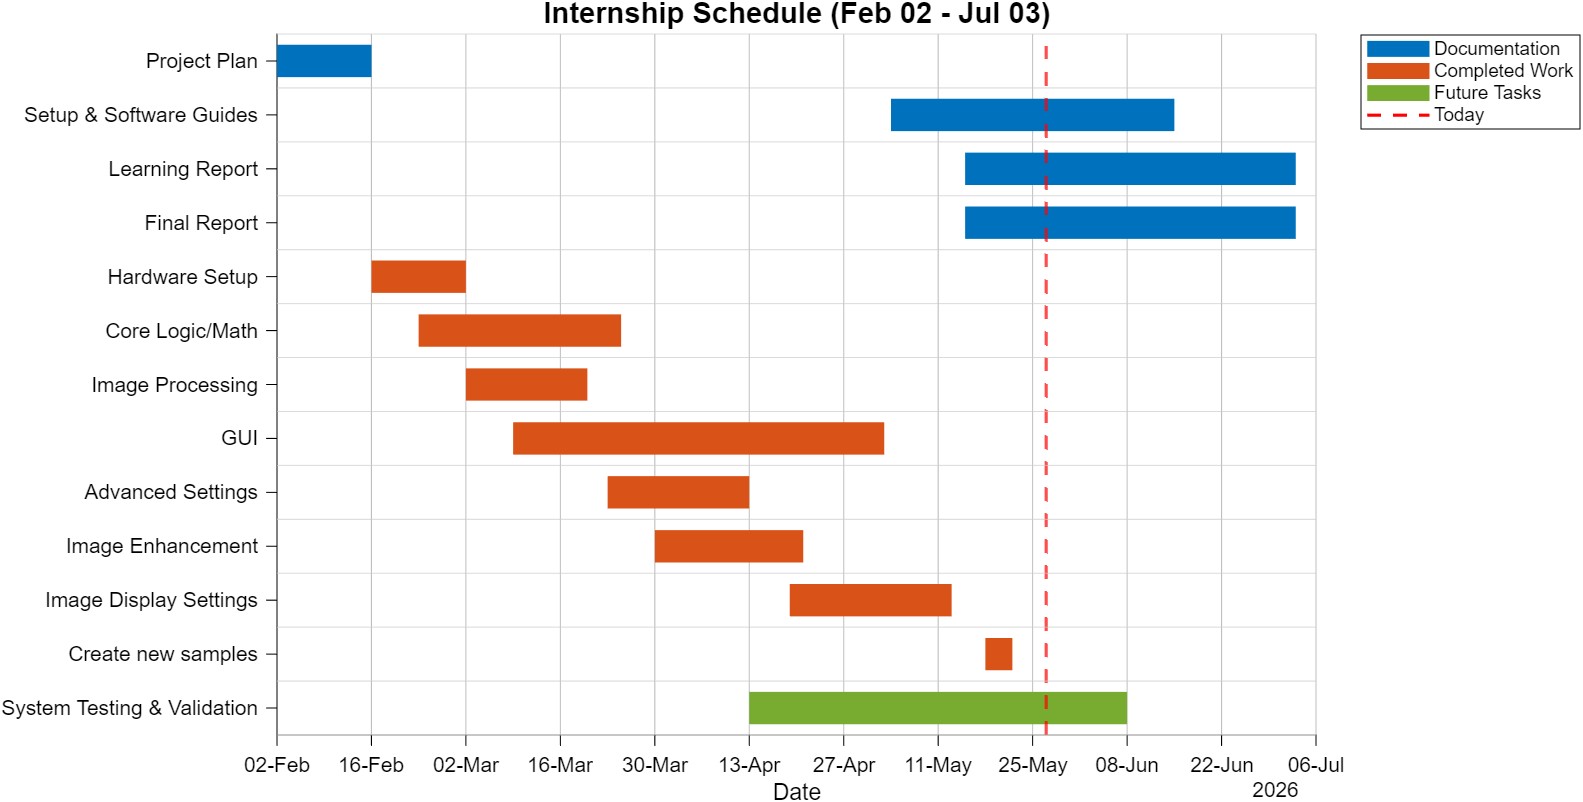
\includegraphics[width=0.9\textheight, height=\textwidth, keepaspectratio]{images/graphs/Gantt.png}}
    \caption{Gantt chart summarizing the sprint structure and key milestones of the development process.}
    \label{fig:gantt_chart}
\end{figure}

\newpage
\section{Kinesis API Object Introspection}
\label{app:kinesis_dir}

Due to the lack of official Python documentation for the Thorlabs Kinesis .NET API, Python's built-in \texttt{dir()} function was utilized to introspect the loaded hardware objects. This reverse-engineering process exposed the necessary methods required to successfully implement closed-loop control and positional readbacks.

\textbf{KCubePiezo (KPZ101) Methods:}
\begin{verbatim}
['CanDeviceLockFrontPanel', 'CanRestorePreSequenceState', 'CheckForIssues', 
'CommsListener', 'CommsListenerFnCallback', 'CommsStatus', 'CommsStatusType', 
'Connect', 'ConnectDevice', 'ConnectionStateChanged', 'ConnectionStateChangedDelegate', 
'ConnectionStateChangedEventArgs', 'ConnectionStates', 'ControlModeUpdate', 
'CreateConnectionToDevice', 'CreateDevice', 'CreateKCubePiezo', 
'DefaultRestorePreSequenceState', 'DeviceErrorUpdate', 'DeviceID', 'DeviceName', 
'DevicePrefix', 'DeviceType', 'DeviceTypeNo', 'DeviceTypes', 'DisableDevice', 
'Disconnect', 'DisconnectTidyUp', 'Dispose', 'EnableCommsListener', 'EnableDevice', 
'Equals', 'Finalize', 'FirmwareVersion', 'FixIssue', 'ForwardException', 
'GetAvailableModes', 'GetConnectionState', 'GetDevParams', 'GetDeviceInfo', 
'GetDeviceName', 'GetDigitalOutputs', 'GetFeedbackLoopPIconsts', 
'GetFrontPanelLocked', 'GetFunctionActor', 'GetFunctionCollection', 
'GetFunctionNames', 'GetFunctionParameters', 'GetFunctionParametersDefinitions', 
'GetHashCode', 'GetIOSettings', 'GetJogParams', 'GetJogSteps', 'GetKCubePiezo', 
'GetLEDBrightness', 'GetListenToStatus', 'GetMMIParams', 'GetMasks', 
'GetMaxOutputVoltage', 'GetMaxTravel', 'GetMinOutputVoltage', 'GetOutputVoltage', 
'GetPercentageTravel', 'GetPiezoConfiguration', 'GetPosition', 
'GetPositionControlMode', 'GetSettings', 'GetSettingsByID', 'GetStatusBits', 
'GetTriggerConfigParams', 'GetType', 'GetVoltageSource', 'HardwareVersion', 
'IdentifyDevice', 'InitializeCoreDevice', 'InitializeDevice', 
'InitializeGenericDevice', 'InitializeGenericPiezo', 'InitializeUSBConnectionState', 
'IsActuator', 'IsBayValid', 'IsClosedLoop', 'IsConnected', 'IsCoreValid', 
'IsDeviceAvailable', 'IsDeviceBusy', 'IsPiezoSettingsValid', 
'IsSetOutputVoltageActive', 'IsSetPositionActive', 'IsSetPositionControlModeActive', 
'IsSettingsInitialized', 'IsSettingsKnown', 'IsSimulation', 'Jog', 
'MaxDigitalOutputId', 'MaxTravelChanged', 'MemberwiseClone', 'MinDigitalOutputId', 
'NativeCoreDevicePtr', 'NativeGenericPiezoPtr', 'Overloads', 'PersistSettings', 
'PiezoConfiguration', 'PiezoDeviceSettings', 'PollingDuration', 
'RaiseDeviceException', 'ReferenceEquals', 'RegisterDevice', 'RequestDevParams', 
'RequestDigitalOutputs', 'RequestFeedbackLoopPIconsts', 'RequestFrontPanelLocked', 
'RequestIOSettings', 'RequestLEDBrightness', 'RequestMMIParams', 
'RequestMaxOutputVoltage', 'RequestOutput', 'RequestPosition', 
'RequestPositionControlMode', 'RequestStatus', 'RequestStatusBits', 
'RequestTriggerConfigParams', 'RequestVoltage', 'RequestVoltageSource', 
'ResetConnection', 'RestorePreSequenceState', 'SerialNo', 'SetDevParams', 
'SetDigitalOutput', 'SetDigitalOutputMode', 'SetDigitalOutputs', 
'SetFeedbackLoopPIconsts', 'SetFrontPanelLock', 'SetIOSettings', 'SetJogSteps', 
'SetLEDBrightness', 'SetLUTwaveParams', 'SetLUTwaveSample', 'SetListenToStatus', 
'SetMMIParams', 'SetMasks', 'SetMaxOutputVoltage', 'SetOutputVoltage', 
'SetPercentageTravel', 'SetPosition', 'SetPositionControlMode', 'SetSettings', 
'SetTriggerConfigParams', 'SetUSBConnectionState', 'SetVoltageSource', 'SetZero', 
'SetZeroOutput', 'SettingsOptions', 'SettingsUpdate', 'SettingsUpdateFnCallback', 
'ShutDown', 'SoftwareVersion', 'StartLUTwave', 'StartPolling', 'Status', 
'StatusChanged', 'StopLUTwave', 'StopPolling', 'StorePreSequenceState', 
'SupportedDevices', 'TestClientWrite', 'ToString', 'USBConnected', 
'UnregisterDevice', 'UpdateActors', 'UsesActuators', 'VerifyDevice', 
'VerifyDeviceConnected', 'VerifySettings', 'WaitForSettingsInitialized']
\end{verbatim}

\textbf{KCubeStrainGauge (KSG101) Methods:}
\begin{verbatim}
['CanDeviceLockFrontPanel', 'CanRestorePreSequenceState', 'CheckForIssues', 
'CommsListener', 'CommsListenerFnCallback', 'CommsStatus', 'CommsStatusType', 
'Connect', 'ConnectDevice', 'ConnectionStateChanged', 'ConnectionStateChangedDelegate', 
'ConnectionStateChangedEventArgs', 'ConnectionStates', 'CreateConnectionToDevice', 
'CreateDevice', 'CreateKCubeStrainGauge', 'DefaultRestorePreSequenceState', 
'DeviceErrorUpdate', 'DeviceID', 'DeviceName', 'DevicePrefix', 'DeviceType', 
'DeviceTypeNo', 'DeviceTypes', 'DisableDevice', 'Disconnect', 'DisconnectTidyUp', 
'DisplayModeUpdate', 'Dispose', 'EnableCommsListener', 'EnableDevice', 'Equals', 
'Finalize', 'FirmwareVersion', 'FixIssue', 'ForwardException', 'GetConnectionState', 
'GetDevParams', 'GetDeviceInfo', 'GetDeviceName', 'GetDigitalOutputs', 
'GetDisplayMode', 'GetFrontPanelLocked', 'GetFunctionActor', 'GetFunctionCollection', 
'GetFunctionNames', 'GetFunctionParameters', 'GetFunctionParametersDefinitions', 
'GetHashCode', 'GetIOsettings', 'GetLEDsetting', 'GetListenToStatus', 'GetMMIParams', 
'GetMasks', 'GetMaxTravel', 'GetReading', 'GetSettings', 'GetSettingsByID', 
'GetStatusBits', 'GetStrainGaugeConfiguration', 'GetTriggerConfigParams', 'GetType', 
'HardwareVersion', 'IdentifyDevice', 'InitializeCoreDevice', 'InitializeDevice', 
'InitializeGenericDevice', 'InitializeGenericPiezo', 'InitializeUSBConnectionState', 
'IsActuator', 'IsBayValid', 'IsConnected', 'IsCoreValid', 'IsDeviceAvailable', 
'IsDeviceBusy', 'IsSettingsInitialized', 'IsSettingsKnown', 'IsSimulation', 
'IsStrainGaugeSettingsValid', 'MaxDigitalOutputId', 'MaxTravelChanged', 
'MemberwiseClone', 'MinDigitalOutputId', 'NativeCoreDevicePtr', 
'NativeGenericStrainGaugePtr', 'Overloads', 'PersistSettings', 'PollingDuration', 
'RaiseDeviceException', 'ReferenceEquals', 'RegisterDevice', 'RequestDevParams', 
'RequestDigitalOutputs', 'RequestDisplayMode', 'RequestFrontPanelLocked', 
'RequestIOsetting', 'RequestLEDsetting', 'RequestMMIParams', 'RequestMaxTravel', 
'RequestReading', 'RequestStatus', 'RequestStatusBits', 'RequestTriggerConfigParams', 
'ResetConnection', 'RestorePreSequenceState', 'SerialNo', 'SetDevParams', 
'SetDigitalOutput', 'SetDigitalOutputMode', 'SetDigitalOutputs', 'SetDisplayMode', 
'SetFrontPanelLock', 'SetIOsettings', 'SetLEDs', 'SetListenToStatus', 'SetMMIParams', 
'SetMasks', 'SetSettings', 'SetTriggerConfigParams', 'SetUSBConnectionState', 
'SetZero', 'SettingsUpdate', 'SettingsUpdateFnCallback', 'ShutDown', 
'SoftwareVersion', 'StartPolling', 'Status', 'StatusChanged', 'StopPolling', 
'StorePreSequenceState', 'StrainGaugeConfiguration', 'StrainGaugeDeviceSettings', 
'StrainGaugeFromDevice', 'SupportedDevices', 'TestClientWrite', 'ToString', 
'USBConnected', 'UnregisterDevice', 'UpdateActors', 'UsesActuators', 'VerifyDevice', 
'VerifyDeviceConnected', 'VerifySettings', 'VerifyStrainGauge', 
'WaitForSettingsInitialized']
\end{verbatim}

\end{document}